% ICML-format version (8 pages + references + appendix). The page geometry emulates the ICML style
% (two columns, 10pt Times, 6.75in x 9in text block); for submission replace the preamble block marked
% STYLE by \usepackage{icml2027} (or the current year) and the ICML title macros. Build: see Makefile.
\documentclass[10pt,twocolumn]{article}
% ---- STYLE (emulation of the ICML layout) ----
\usepackage[letterpaper,textwidth=6.75in,textheight=9in,top=1in,columnsep=0.25in]{geometry}
\usepackage{times}
\usepackage[T1]{fontenc}
% ---- end STYLE ----
\usepackage{amsmath,amssymb,amsthm}
\usepackage{graphicx}
\usepackage{booktabs}
\usepackage[round]{natbib}
\usepackage{xcolor}
\usepackage[colorlinks=true,linkcolor=blue!50!black,citecolor=blue!50!black,urlcolor=blue!50!black]{hyperref}
\usepackage{enumitem}
\usepackage{microtype}
\usepackage{caption}
\captionsetup{font=small,labelfont=bf}

\newtheorem{proposition}{Proposition}
\newtheorem{lemma}{Lemma}
\newtheorem{definition}{Definition}
\theoremstyle{remark}
\newtheorem{remark}{Remark}
\newcommand{\pending}[1]{\textcolor{red}{[#1]}}
\newcommand{\R}{\mathbb{R}}
\newcommand{\tr}{\operatorname{tr}}
\newcommand{\MS}{\operatorname{MS}}
\graphicspath{{../../figures/}}

\title{\vspace{-2.2em}\textbf{Flat in the Wrong Coordinates:\\Optimizer-Induced Symmetry Drift Biases Sharpness Comparisons Between Adam and SGD}\vspace{-0.6em}}
\author{Anonymous Authors\vspace{-1.2em}}
\date{}

\begin{document}
\maketitle

\begin{abstract}
Whether Adam or SGD finds flatter minima is often measured and rarely agreed upon. We show that such comparisons mix two factors: the geometry of the learned function, and the point of the network's rescaling-symmetry orbit at which that function happens to be represented. For the Hessian trace, which in ReLU networks without normalization layers equals the Gauss--Newton trace, the split is exact: raw trace $=$ \emph{minimum sharpness} $\times$ \emph{orbit excess}. We prove that SGD cannot move along these orbits at first order, whereas Adam and other diagonally preconditioned methods drift along them at a rate approximately $\propto\eta\sqrt{\text{fan-in}}$ at small learning rates and settle near the trace-minimizing coordinates. In 162 loss-matched runs of MLPs and a small CNN, with up to 17 measures, the resulting coordinate factor ($\approx2\times$ on a CIFAR-10 MLP) is as large as the functional differences being measured: it reverses the Adam--SGD flatness ranking on a CIFAR-10 MLP, flips it during training on MNIST, and masks a large difference on a CNN, and it does not grow with depth. A causal intervention that undoes Adam's drift roughly doubles raw sharpness and leaves minimum sharpness unchanged; further controls suggest that the drift also helps Adam train in noisy settings. With label noise, the orbit becomes an exactly computable testbed for implicit regularization: SGD drifts toward minimum trace and Adam toward minimum $\sum_i\sqrt{G_{ii}}$, as theory predicts, in all 32 runs of each (16 independent initializations). With BatchNorm (an MLP and ResNet-18 on full CIFAR-10), raw measures follow weight norms set by the learning rate and weight decay, and the direction of the invariant verdict differs between the two networks. Cross-optimizer flatness comparisons should report rescaling-invariant measures, or at least the orbit excess.
\end{abstract}

%===============================================================================
\section{Introduction}
%===============================================================================
The idea that flat minima generalize better than sharp ones \citep{hochreiter1997flat,keskar2017large} motivates both analysis tools and optimizers such as SAM \citep{foret2021sam}. A recurring empirical question is \emph{which optimizer finds flatter minima}. Adaptive methods such as Adam \citep{kingma2015adam} are often reported to generalize worse than SGD \citep{wilson2017marginal}, and a popular explanation is that they converge to sharper minima \citep{zhou2020towards}. Measurements nevertheless disagree, and recent theory suggests that Adam and SGD implicitly minimize \emph{different} notions of sharpness \citep{li2025adam}.

This paper began as an attempt to answer that question with a standard tool, the relative loss increase under isotropic Gaussian weight noise. The preliminary result was that Adam's minima appeared \emph{flatter} than SGD's on MNIST and CIFAR-10. It was an artifact, and the reason turned out to be general and mechanistic.

\citet{dinh2017sharp} showed that function-preserving reparameterizations of ReLU networks can make any minimum arbitrarily sharp or flat. A common reply is that no optimizer performs such reparameterizations. Our central finding is that \textbf{Adam does}: it moves systematically along the network's rescaling symmetries and settles near the coordinates in which its solution has close to the smallest Hessian trace, whereas SGD provably cannot move along them at first order. A raw sharpness comparison between Adam and SGD therefore compares two functions \emph{and} two positions on their symmetry orbits, and the second factor is often the larger one (Fig.~\ref{fig:teaser}).

\begin{figure}[t]
\centering
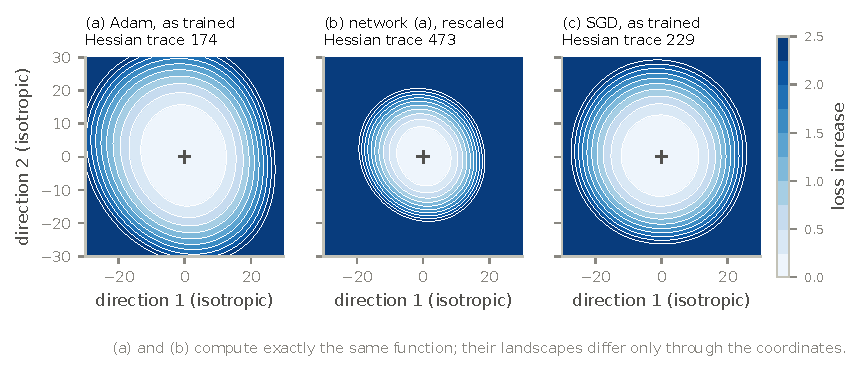
\includegraphics[width=\columnwidth]{fig0_same_function.pdf}
\caption{\textbf{Same function, different landscape.} Loss slices along the same two random directions around (a) an MLP trained with Adam, (b) the \emph{identical function} after rescaling every hidden neuron to the minimum-norm representative, and (c) an MLP trained with SGD (CIFAR-10, training loss $\le0.01$). In its own coordinates Adam's solution looks flatter than SGD's; a function-preserving change of coordinates makes it $2.7\times$ sharper.}
\label{fig:teaser}
\end{figure}

\paragraph{Contributions.}
\begin{itemize}[leftmargin=1.1em,itemsep=1pt,topsep=2pt]
\item \textbf{A diagnostic decomposition} (\S\ref{sec:setup}): writing the trace as the minimum sharpness of the function \citep{ibayashi2021minimum} times an orbit excess $\ge1$ is immediate from the definitions; we use it to attribute cross-optimizer differences, and show that it applies to the Hessian trace itself in ReLU networks without normalization (Lemma~\ref{lem:diag}).
\item \textbf{A mechanism with a proof and a scaling law} (\S\ref{sec:mechanism}): the first-order drift of the conserved quantity $\|w_{\mathrm{in}}\|^2-\|w_{\mathrm{out}}\|^2$ vanishes for plain SGD, is second order for momentum, is proportional to the radius for SAM, and is generically nonzero for diagonal preconditioners, scaling as $\eta\sqrt{\text{fan-in}}$.
\item \textbf{A loss-matched audit} (\S\ref{sec:audit}): the coordinate factor reverses, flips or masks optimizer rankings depending on the size of the true difference, at every depth we test (MLPs with 1--8 hidden layers).
\item \textbf{A causal test} (\S\ref{sec:intervention}): removing Adam's drift doubles raw sharpness and leaves invariant sharpness unchanged; holding Adam at different orbit points suggests the drift also helps it train (one CIFAR-10 MLP).
\item \textbf{An empirical test of implicit-regularization theory} (\S\ref{sec:labelnoise}): with label noise, SGD and Adam drift toward the orbit points predicted by \citet{damian2021label} and \citet{li2025adam}, in nonlinear networks where the destinations are known exactly. This tests their theory; it does not extend it.
\end{itemize}

%===============================================================================
\section{Related work}
%===============================================================================
\textbf{Sharpness and generalization.} Many sharpness measures exist \citep{keskar2017large,jiang2020fantastic}, including scale-aware variants \citep{kwon2021asam,tsuzuku2020normalized,petzka2021relative,rangamani2019scale,li2018visualizing}; their correlation with generalization is fragile \citep{jiang2020fantastic,andriushchenko2023modern,kaur2023maximum}. Hessian-based flatness is not invariant to reparametrization unless the metric is made explicit \citep{kristiadi2023geometry,ahmed2026fisher}. \citet{ibayashi2021minimum} proposed \emph{minimum sharpness}, the minimal trace over rescaling-equivalent parameterizations. We use it and show that the gap between raw trace and minimum sharpness is systematically optimizer-dependent. \citet{zhang2021flatness} observed that Adam can break the flatness--generalization link; we identify a mechanism behind such breakdowns.
\textbf{Symmetries and conservation laws.} Gradient flow on homogeneous networks conserves $\|w_{\mathrm{in}}\|^2-\|w_{\mathrm{out}}\|^2$ per unit \citep{du2018algorithmic}; finite learning rates, momentum and weight decay break such laws \citep{kunin2021neural,marcotte2023abide,marcotte2024keep}, and minibatch noise slowly moves SGD along exponential symmetries \citep{ziyin2023law,ziyin2024parameter}. \citet{singh2026loss} showed that coordinate-wise methods are not equivariant under the gauge symmetry of matrix factorization; Proposition~\ref{prop:drift} is the analogue for ReLU rescaling. Symmetry teleportation moves parameters along orbits deliberately \citep{zhao2022teleport,zhao2024improving,lebeurrier2026path}; \citet{saul2023weight} rebalances norms by per-unit rescaling, and discrete gradient descent breaks the conservation laws at second order \citep{medeiros2026conservation}. Recent preprints report that Adam drifts along symmetry orbits and propose equivariant variants \citep{shirodkar2026dead}, and that unbalancing paired norms by a function-preserving rescaling degrades later Transformer training even with transformed AdamW moments \citep{kim2026same}, paralleling our Adam-Q results. Our contribution is to show where the drift leads, how large it is, and that it biases optimizer comparisons enough to change conclusions.
\textbf{Implicit sharpness regularization.} Label-noise SGD implicitly minimizes $\tr H$ \citep{blanc2020implicit,damian2021label}, Adam minimizes $\tr\,\mathrm{diag}(H)^{1/2}$ \citep{li2025adam}, and gradient methods train at the edge of stability \citep{cohen2021eos,cohen2022adaptive}.

%===============================================================================
\section{Rescaling orbits, a conservation law, and minimum sharpness}\label{sec:setup}
%===============================================================================
Consider a network of linear or convolutional layers with positively homogeneous activations (ReLU, max-pooling). For a hidden unit $j$ let $a_j$ collect its incoming weights and bias and $c_j$ its outgoing weights. The map $T^{(j)}_s:(a_j,c_j)\mapsto(e^{s}a_j,e^{-s}c_j)$ leaves the network function unchanged; such maps generate the \emph{rescaling orbit} of $\theta$.

\begin{lemma}[Euler identity]\label{lem:euler}
For any loss $\ell$ that depends on $\theta$ only through the network function, including any minibatch loss, $\langle a_j,\nabla_{a_j}\ell\rangle=\langle c_j,\nabla_{c_j}\ell\rangle$ for every hidden unit $j$.
\end{lemma}
\begin{proof}
$s\mapsto\ell(T^{(j)}_s\theta)$ is constant; differentiate at $s=0$.
\end{proof}

Let $Q_j=\|a_j\|^2-\|c_j\|^2$. For an update $\theta^+=\theta+u$, expanding the squares gives the \emph{exact} decomposition
\begin{equation}\label{eq:decomp}
\Delta Q_j=\underbrace{2\big(\langle a_j,u_{a_j}\rangle-\langle c_j,u_{c_j}\rangle\big)}_{D^{(1)}_j\ \text{(first order)}}+\underbrace{\|u_{a_j}\|^2-\|u_{c_j}\|^2}_{D^{(2)}_j\ \text{(second order)}}.
\end{equation}

\begin{proposition}\label{prop:drift}
\textbf{(a) SGD.} For $u=-\eta\nabla\ell_B$ on any minibatch $B$, $D^{(1)}_j=0$ exactly.
\textbf{(b) Heavy-ball momentum.} $D^{(1)}_j$ is a sum of terms each containing a parameter difference $\theta_t-\theta_{t-k}=O(\eta)$, so the drift is second order in $\eta$ (with a $\beta$-dependent prefactor that we do not bound).
\textbf{(c) Diagonal preconditioning} (Adam, RMSProp, sign descent). For $u=-\eta P^{-1}m$ with diagonal $P\succ0$, $D^{(1)}_j=-2\eta\big(\langle a_j,P_a^{-1}m_a\rangle-\langle c_j,P_c^{-1}m_c\rangle\big)$, which is generically nonzero. For sign descent, $D^{(1)}_j=2\eta(\rho_a\|a_j\|_1-\rho_c\|c_j\|_1)$ with $\rho_x\in[-1,1]$ the $\ell_1$-weighted net fraction of coordinates moving away from zero.
\textbf{(d) SAM} with radius $r$: $D^{(1)}_j=2\eta(\langle\varepsilon_{a_j},\tilde g_a\rangle-\langle\varepsilon_{c_j},\tilde g_c\rangle)$, with $\varepsilon$ the ascent step and $\tilde g$ the gradient at $\theta+\varepsilon$: first order in $\eta$, proportional to $r$.
\end{proposition}
\begin{proof}
(a) Lemma~\ref{lem:euler} for $\ell_B$. (b) Lemma~\ref{lem:euler} at each $t-k$, subtracted. (c) Substitution. (d) Lemma~\ref{lem:euler} at $\theta+\varepsilon$.
\end{proof}
The proposition is exact for one discrete step. It assumes the loss depends on $\theta$ only through the network function ($a_j$ includes the bias) and no weight decay, which adds $-2\eta\lambda Q_j$ for SGD; none of the MLP or CNN runs uses it. $D^{(2)}_j$ is not zero in general, so SGD can still drift slowly (\S\ref{sec:labelnoise}).

\begin{remark}[Why $\sqrt{\text{fan-in}}$]\label{rem:fanin}
SGD moves each weight in proportion to its partner weights, which is what keeps $Q_j$ fixed. Sign-like updates move every coordinate by $\approx\eta$; since $\|x\|_1\approx\kappa\sqrt{d}\|x\|_2$ for dense vectors, a unit whose fan-in exceeds its fan-out drifts toward large incoming norm at a rate $\propto\eta\sqrt{d_{\mathrm{in}}}$. Adam behaves like sign descent when gradient noise is small \citep{balles2018dissecting,bernstein2018signsgd}.
\end{remark}

\textbf{Exact transport of curvature.} A rescaling acts as $\theta'=D\theta$ with $D$ diagonal and positive, so the Hessian and the Gauss--Newton matrix $G$ transform \emph{exactly}, $H(\theta')=D^{-1}H(\theta)D^{-1}$ and $G(\theta')=D^{-1}G(\theta)D^{-1}$: $\mathrm{diag}(G)$ anywhere on the orbit follows from $\mathrm{diag}(G)$ at $\theta$.

\begin{lemma}\label{lem:diag}
For networks of affine layers and piecewise-linear activations and pooling (ReLU, max-pooling) without normalization layers, and a loss twice differentiable in the outputs, $\mathrm{diag}\,H=\mathrm{diag}\,G$ almost everywhere; hence $\tr H=\tr G$.
\end{lemma}
\begin{proof}
$H=G+\frac1N\sum_{n,k}\frac{\partial\ell}{\partial f_k}\nabla^2f_k$, and with the activation pattern and all other parameters fixed $f$ is affine in each single parameter, so the second term has a zero diagonal.
\end{proof}
$H\ne G$ off the diagonal, so we compute $\lambda_{\max}$ from $H$; the trace, $\MS_p$ and the decomposition below are the same for both in our MLPs and CNN (checked to $5\times10^{-16}$ in float64; the Hutchinson $\tr H$ matches the exact $\tr G$ within its sampling error at all 913 MLP checkpoints). With BatchNorm the lemma fails (diagonals differ by up to $94\%$), so \S\ref{sec:bn} uses Hessian-based measures only.

\begin{definition}[Minimum sharpness and orbit excess]
Following \citet{ibayashi2021minimum}, for $p>0$ let $\MS_p(\theta)=\min_{\theta'\in\mathrm{orbit}(\theta)}\sum_iG_{ii}(\theta')^{p}$. $\MS_1$ is the minimal trace and $\MS_{1/2}$ the orbit minimum of Adam's implicit regularizer \citep{li2025adam}. The \emph{orbit excess} is $E=\tr G/\MS_1\ge1$, so that
\begin{equation}\label{eq:factor}
\tr G(\theta)=\underbrace{\MS_1(\theta)}_{\text{orbit minimum}}\times\underbrace{E(\theta)}_{\text{orbit excess}}.
\end{equation}
\end{definition}
$\MS_1$ is constant on the rescaling orbit (an orbit invariant, not a property of the input--output function: redundant units can represent one function on several orbits), so a comparison of $\log\tr G$ splits \emph{exactly} into a orbit-minimum term and a coordinate term. The objective is a posynomial in the unit scales, convex in their logarithms; exact coordinate descent has the closed form $c_j^{2p}=\sqrt{A_j/B_j}$, where $A_j$ and $B_j$ aggregate unit $j$'s incoming and outgoing curvature. At $p=1$ the optimum is \emph{curvature balance}, $A_j=B_j$, not the norm balance of the minimum-norm point. We compute $\mathrm{diag}(G)$ exactly (one backward pass per class for MLPs, per-sample gradients for CNNs); $\MS_p$ then takes milliseconds.

%===============================================================================
\section{Experimental protocol}\label{sec:protocol}
%===============================================================================
\textbf{Data and models.} MNIST and CIFAR-10 with a class-balanced 10k-example training subset, the full test set and per-channel standardization; an MLP (in--128--64--10, the architecture of the original study) and a small CNN (two $3{\times}3$ conv layers with max-pooling, then two dense layers), without normalization layers.
\textbf{Optimizers.} SGD, SGD with momentum $0.9$ (SGD+M), SAM ($\rho=0.05$) and Adam, each with two base learning rates and batch sizes $\{32,128,512\}$ ($\eta=\eta_0\sqrt{B/32}$) and three seeds: 72 runs per dataset, with rates chosen by a calibration sweep (App.~\ref{app:calibration}).
\textbf{Loss matching.} Fixed-epoch comparisons conflate the optimizer with how far training has progressed, and cross-entropy curvature shrinks with the loss. Each run is therefore measured when its full training loss first falls below $\{1,0.3,0.1,0.03,0.01\}$, and only checkpoints at the same target are compared.
\textbf{Measures.} On 4096 training examples we compute 17 measures (App.~\ref{app:measures}). \emph{Coordinate-dependent:} the original metric (relative isotropic sharpness on the test set), isotropic average sharpness, the Hessian trace (Hutchinson estimate, and exactly as $\tr G$), $\lambda_{\max}$, worst-case SAM sharpness, $\sum_i\sqrt{G_{ii}}$, and several of these at the minimum-norm point. \emph{Rescaling-invariant:} $\MS_1$, $\MS_{1/2}$, multiplicative average sharpness, ASAM \citep{kwon2021asam} and $\sum_iw_i^2G_{ii}$. Filter-normalized sharpness \citep{li2018visualizing} is invariant to row scaling only: a random neuron rescaling changes it $9.5\times$.
\textbf{Statistic.} $P(S_{\mathrm{Adam}}<S_X)$ over all Adam/$X$ configuration pairs sharing a seed and loss target (108 pairs; $0.5$ = no difference), and the exact split of $\log_2(\tr G_{\mathrm{Adam}}/\tr G_X)$ into function and coordinate terms via~\eqref{eq:factor}. 95\% intervals from a cluster bootstrap over runs.

%===============================================================================
\section{Results}
%===============================================================================
\subsection{Adam drifts along the orbit; SGD does not}\label{sec:mechanism}
\begin{figure*}[t]
\centering
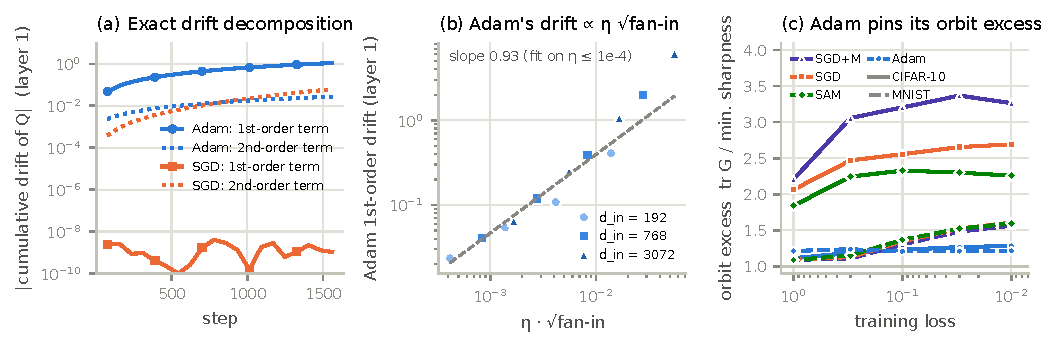
\includegraphics[width=\textwidth]{fig2_mechanism.pdf}
\caption{\textbf{Mechanism.} \textbf{(a)} Exact decomposition~\eqref{eq:decomp} of the cumulative drift of $Q_j$ (CIFAR-10 MLP). SGD's first-order term is zero up to round-off; Adam's dominates its own second-order term. \textbf{(b)} Adam's first-order drift after 20 epochs against $\eta\sqrt{\text{fan-in}}$ (four learning rates, three input resolutions). \textbf{(c)} Orbit excess at matched training loss (median of 18 runs; solid: CIFAR-10, dashed: MNIST).}
\label{fig:mechanism}
\end{figure*}

We log both terms of~\eqref{eq:decomp} at every step on the CIFAR-10 MLP across learning rates and input resolutions (66 runs). SGD's first-order term is below $3{\times}10^{-7}$ in every run, zero up to round-off. Adam's is $0.02$--$6.2$ and exceeds its own second-order term by $23$--$800\times$ (Fig.~\ref{fig:mechanism}a); SGD+M drifts only at second order. A log-linear fit gives exponents $0.91$ for $\eta$ and $0.94$ for $\sqrt{d_{\mathrm{in}}}$ at small $\eta$ (Fig.~\ref{fig:mechanism}b), as Remark~\ref{rem:fanin} predicts. RMSprop and plain sign descent behave the same way (App.~\ref{app:drift}).

\textbf{Where the drift leads.} At initialization the CIFAR-10 MLP has orbit excess $E=3.66$. Adam moves to a median $E=1.11$--$1.28$ at every loss level, and across all 90 Adam checkpoints $E\in[1.08,1.48]$, against $[1.45,4.89]$ for the other optimizers, whose median excess is $1.8$--$3.4$ (Fig.~\ref{fig:mechanism}c). The same holds on MNIST (Adam $1.21$--$1.24$), in MLPs with 1 to 8 hidden layers (Adam $1.16$--$1.39$, SGD and SGD+M $1.50$--$2.15$; App.~\ref{sec:depth-full}), and from different starting points of the same orbit (\S\ref{sec:labelnoise}).

\subsection{The coordinate factor reverses, flips or masks rankings}\label{sec:audit}
\begin{figure*}[t]
\centering
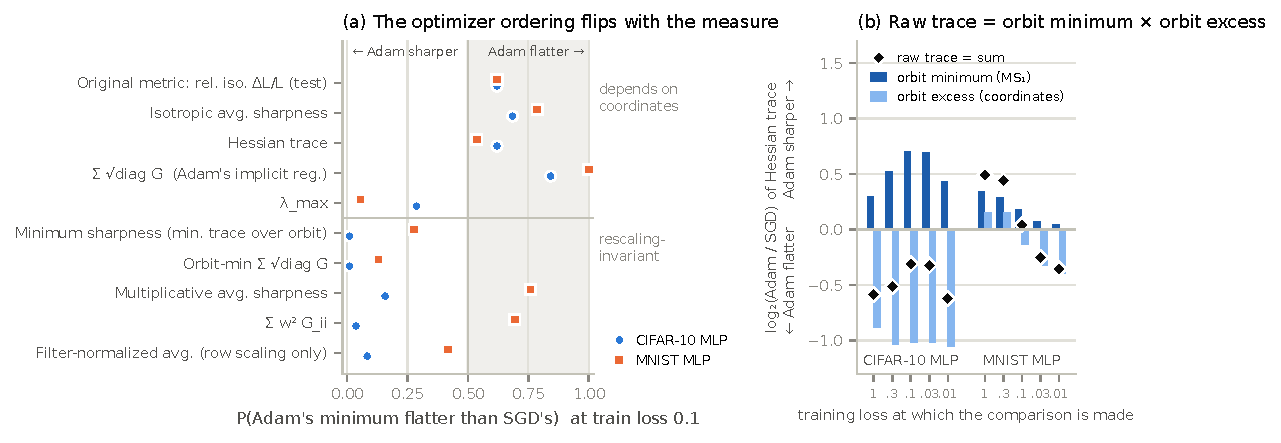
\includegraphics[width=0.92\textwidth]{fig1_flip.pdf}
\caption{\textbf{(a)} Probability that Adam's minimum is rated flatter than SGD's (108 loss-matched pairs, training loss $0.1$). \textbf{(b)} Exact split~\eqref{eq:factor} of the Adam/SGD trace ratio into a orbit-minimum term and a coordinate term at each matched loss. On CIFAR-10 the coordinate term favours Adam by $\approx2\times$ and outweighs the orbit-minimum term; on MNIST it changes sign during training.}
\label{fig:flip}
\end{figure*}

\textbf{CIFAR-10: a reversal.} At every matched loss, Adam is rated flatter than SGD by the original metric ($P=0.62$--$0.67$), isotropic sharpness ($0.69$--$0.75$), the Hessian trace ($0.62$--$0.74$) and $\sum_i\sqrt{G_{ii}}$ ($0.84$--$1.00$), and sharper by minimum sharpness ($0.01$--$0.22$), $\MS_{1/2}$, multiplicative sharpness and $\sum_iw_i^2G_{ii}$ (Fig.~\ref{fig:flip}a, Table~\ref{tab:flip}). The disagreement is well determined: $P_{\tr G}-P_{\MS_1}=+0.63$ $[+0.43,+0.81]$ at loss $0.1$. The exact split explains it: the orbit-minimum term is $+0.43$ to $+0.71$ bits (Adam sharper) and the coordinate term $-1.02$ to $-1.05$ bits, a factor of almost exactly $2$ in Adam's favour at every loss (Fig.~\ref{fig:flip}b). Against SAM, the one optimizer designed to seek flat minima, raw trace is inconclusive ($P=0.44$--$0.60$) because a large orbit-minimum term in SAM's favour is cancelled by the coordinate term; invariant measures identify SAM as clearly flatter ($P=0.00$--$0.23$).

\textbf{MNIST: a flip during training.} The initial excess is smaller. Early on SGD's excess is \emph{below} Adam's and raw measures rate Adam sharper ($P=0.06$ for the trace at loss $0.3$); as SGD's excess grows the coordinate term turns ($-0.40$ bits at loss $0.01$) and the raw ordering flips ($P=0.80$), while the orbit-minimum term never favours Adam.

\begin{figure*}[t]
\centering
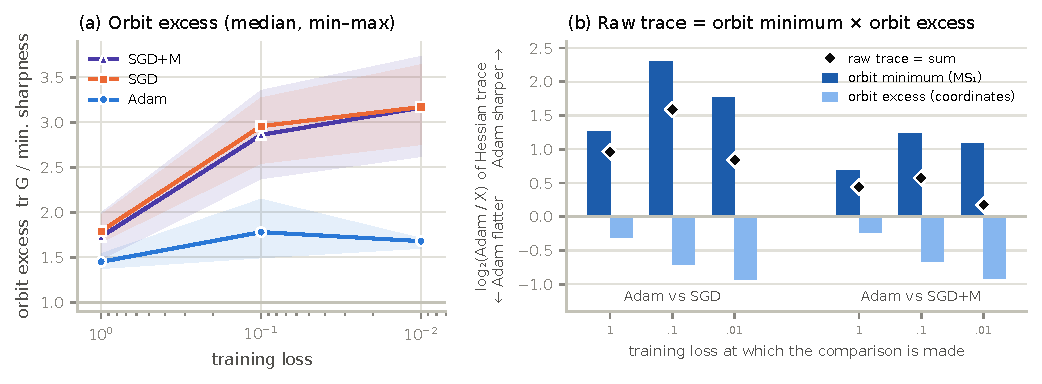
\includegraphics[width=0.85\textwidth]{fig6_cnn.pdf}
\caption{\textbf{CNN on CIFAR-10.} \textbf{(a)} Orbit excess at matched training loss; rescaling acts on convolutional channels, through max-pooling and the flatten into the dense layer. \textbf{(b)} Exact split of the Adam/X trace ratio. On this network Adam's solutions are sharper in orbit-minimized sharpness, and the coordinate term, which again favours Adam and grows during training, hides most of that difference.}
\label{fig:cnn}
\end{figure*}

\textbf{CNN: a mask.} On the CNN Adam's solutions are clearly sharper in orbit-minimized sharpness ($+1.27$ to $+2.30$ bits against SGD; every invariant measure gives $P=0.00$), and the coordinate term again favours Adam and grows during training ($-0.31$ to $-0.93$ bits). Against SGD+M it hides most of the difference: raw measures are inconclusive ($P=0.25$--$0.50$) although Adam is about $2\times$ sharper (Fig.~\ref{fig:cnn}).

\begin{figure}[t]
\centering
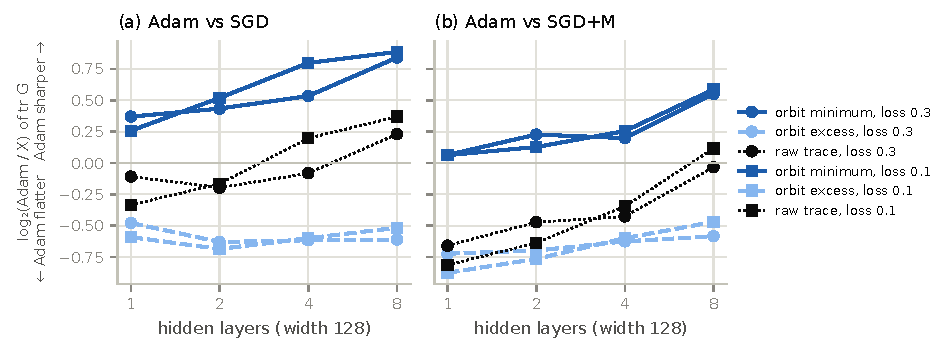
\includegraphics[width=\columnwidth]{fig10_depth.pdf}
\caption{\textbf{Depth.} Exact split~\eqref{eq:factor} of the Adam/X trace ratio for CIFAR-10 MLPs with 1--8 hidden layers of width 128 (three seeds each). The coordinate term is about the same at every depth; the orbit-minimum term grows with depth, so the coordinate factor reverses the raw ordering in shallow networks and masks the difference in deep ones.}
\label{fig:depth}
\end{figure}

\textbf{Depth.} In MLPs with 1, 2, 4 and 8 hidden layers the coordinate term is the same at every depth ($-0.48$ to $-0.74$ bits against SGD), while the orbit-minimum term grows ($+0.26$--$+0.37$ bits at depth 1, $+0.76$--$+0.89$ at depth 8): the factor reverses the ordering in shallow networks and masks it in deep ones (Fig.~\ref{fig:depth}).

\begin{table}[t]
\centering
\footnotesize
\caption{$P(\text{Adam rated flatter than }X)$ at matched training loss $L$ (108 pairs per cell). Below $0.5$: Adam rated sharper.}
\label{tab:flip}
\setlength{\tabcolsep}{2.4pt}
\begin{tabular}{lcccccc}
\toprule
& \multicolumn{3}{c}{CIFAR-10 vs SGD} & \multicolumn{3}{c}{MNIST vs SGD}\\
\cmidrule(lr){2-4}\cmidrule(lr){5-7}
Measure & $0.3$ & $0.1$ & $0.01$ & $0.3$ & $0.1$ & $0.01$\\
\midrule
Original metric & 0.66 & 0.62 & 0.67 & 0.27 & 0.62 & 0.97\\
Isotropic average & 0.74 & 0.69 & 0.75 & 0.41 & 0.79 & 0.90\\
Hessian trace (Hutch.) & 0.74 & 0.62 & 0.74 & 0.06 & 0.54 & 0.83\\
$\sum_i\sqrt{G_{ii}}$ & 1.00 & 0.84 & 0.92 & 1.00 & 1.00 & 1.00\\
$\lambda_{\max}$ & 0.37 & 0.29 & 0.45 & 0.00 & 0.06 & 0.32\\
\midrule
$\MS_1$ (inv.) & 0.06 & 0.01 & 0.22 & 0.09 & 0.28 & 0.44\\
$\MS_{1/2}$ (inv.) & 0.03 & 0.01 & 0.19 & 0.00 & 0.13 & 0.31\\
Multiplicative (inv.) & 0.31 & 0.16 & 0.25 & 0.57 & 0.76 & 0.73\\
$\sum_iw_i^2G_{ii}$ (inv.) & 0.18 & 0.04 & 0.24 & 0.54 & 0.69 & 0.84\\
Filter-norm.\ (part.) & 0.14 & 0.08 & 0.06 & 0.47 & 0.42 & 0.20\\
\bottomrule
\end{tabular}
\end{table}

\textbf{Caveats.} Invariant measures remove the coordinate artifact but need not agree with each other: on MNIST, the elementwise-relative family rates Adam flatter late in training while minimum sharpness does not. We therefore make no universal claim that Adam's minima \emph{are} sharper. $\lambda_{\max}$ rates Adam sharper even in raw coordinates; it is dominated by a few outlier directions, whereas the drift reshapes the bulk of the diagonal. The trace at the minimum-norm point is also orbit-invariant but disagrees with $\MS_1$ ($P=0.31$--$0.56$): the two evaluate curvature at different canonical points (norm vs.\ curvature balance), so orbit invariance alone does not settle the comparison.

\begin{figure}[t]
\centering
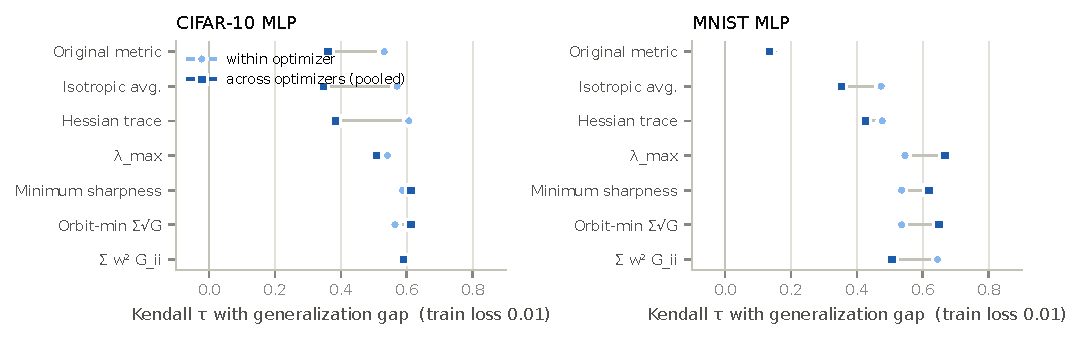
\includegraphics[width=\columnwidth]{fig5_generalization.pdf}
\caption{Kendall $\tau$ between each measure and the generalization gap (train minus test accuracy) at training loss $0.01$, computed within each optimizer (averaged over the four optimizers) and pooled across optimizers. Raw measures lose predictive power when models from different optimizers are ranked together; minimum sharpness does not.}
\label{fig:gen}
\end{figure}

\begin{table*}[t]
\centering
\footnotesize
\caption{The original protocol, re-run with five seeds: raw $[0,1]$ inputs, full training sets, 20 epochs, batch size 64, SGD $\eta=0.01$ vs.\ Adam $\eta=0.001$, measured once at the end (mean $\pm$ s.d.). The ``Adam is flatter'' result replicates. On CIFAR-10 it is almost entirely the coordinate factor; on MNIST it is a training-loss mismatch.}
\label{tab:replication}
\setlength{\tabcolsep}{6pt}
\begin{tabular}{lcccc}
\toprule
& \multicolumn{2}{c}{CIFAR-10} & \multicolumn{2}{c}{MNIST}\\
\cmidrule(lr){2-3}\cmidrule(lr){4-5}
& SGD & Adam & SGD & Adam\\
\midrule
Original metric $\Delta L/L$ (test) & $0.034\pm0.002$ & $0.012\pm0.003$ & $0.040\pm0.008$ & $0.014\pm0.010$\\
Training loss at measurement & $1.42\pm0.05$ & $1.29\pm0.02$ & $0.136\pm0.005$ & $0.008\pm0.004$\\
Test accuracy & $0.475\pm0.016$ & $0.496\pm0.005$ & $0.957\pm0.001$ & $0.978\pm0.002$\\
Hessian trace ($=\tr G$) & $1004\pm31$ & $395\pm19$ & $96.2\pm1.2$ & $9.7\pm3.1$\\
\quad minimum sharpness $\MS_1$ (function) & $353\pm18$ & $320\pm11$ & $72.0\pm1.1$ & $8.0\pm2.4$\\
\quad orbit excess $E$ (coordinates) & $2.85$ & $1.23$ & $1.34$ & $1.21$\\
Filter-normalized average, scale $0.1$ ($\times10^{4}$) & $78\pm34$ & $207\pm36$ & $41\pm9$ & $17\pm7$\\
Multiplicative average, $\sigma=0.1$ ($\times10^{4}$) & $109\pm21$ & $263\pm13$ & $61\pm13$ & $11\pm3$\\
\bottomrule
\end{tabular}
\end{table*}

\textbf{Consequences.} Removing the coordinate factor raises the \emph{cross-optimizer} Kendall correlation between sharpness and the generalization gap from $0.38$ to $0.61$ (CIFAR-10) and $0.47$ to $0.62$ (MNIST) and leaves within-optimizer correlations unchanged (Fig.~\ref{fig:gen}). Re-running the original fixed-epoch protocol shows that its ``Adam is flatter'' result came from the coordinate factor on CIFAR-10 and from a $17\times$ training-loss mismatch on MNIST (Table~\ref{tab:replication}).

\subsection{Causal test: removing and relocating Adam's drift}\label{sec:intervention}
\begin{figure}[t]
\centering
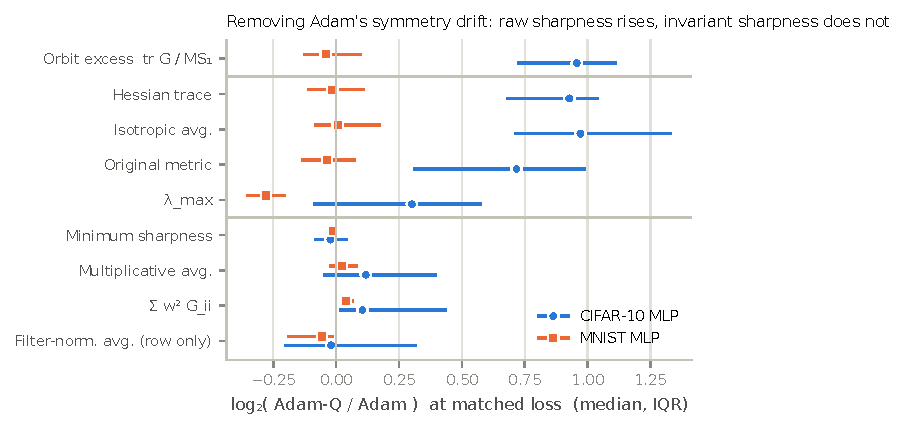
\includegraphics[width=\columnwidth]{fig3_intervention.pdf}
\caption{\textbf{Causal test.} Adam-Q / Adam at matched training loss (median, IQR). On CIFAR-10 removing the drift doubles the orbit excess and every raw trace-type measure; invariant measures do not move. On MNIST, whose conserved coordinates are already near the orbit minimum, nothing moves.}
\label{fig:intervention}
\end{figure}

\emph{Adam-Q} runs Adam and, after every step, applies the function-preserving rescaling that restores each unit's $Q_j$ to its initial value (per-unit closed form, two layer-wise sweeps; residual below $10^{-3}$ of $\max|Q^{(0)}|$), transforming Adam's moments covariantly. It optimizes the same loss and differs from Adam only through Adam's lack of rescaling-equivariance. Comparing loss-matched checkpoints of the same configurations (Fig.~\ref{fig:intervention}): on CIFAR-10 the orbit excess rises from $1.18$ to $2.35$, $\tr G$ by a median factor of $1.91$ (IQR $1.63$--$2.04$), the original metric by $1.64$, while $\MS_1$ moves by $0.98$ and test accuracy by $0.995$. Against SGD, Adam-Q is no longer rated flatter ($P$ by $\tr G$ drops from $0.64$--$0.75$ to $0.21$--$0.35$). On MNIST the excess barely changes and neither do the raw measures: a dose--response.

\textbf{The drift also helps Adam train.} In the six noisiest CIFAR-10 configurations Adam-Q stalls: it never gets below loss $\approx0.05$ within 300 epochs, while Adam reaches $0.01$ by epoch $\approx55$. Holding Adam at chosen orbit points by function-preserving teleports every 100 steps separates the intervention from the position. Held at the minimum-trace point (excess $1.00$--$1.01$), Adam trains as fast as Adam (loss $0.01$ in 51--61 vs.\ 52--67 epochs). Held at the minimum-norm point, where Adam-Q ends up (excess $2.1$--$2.8$), it stalls like Adam-Q in every noisy run (final loss $0.17$--$0.30$). If Adam's update noise is roughly uncorrelated across coordinates with equal variance (an assumption), the loss it injects, $\frac12\tr(HC)$, scales with the trace in its \emph{current} coordinates; this suggests the drift lowers Adam's own noise floor, a heuristic that predicts the direction of the effect but not its size.

\textbf{Adam's coordinates do not help SGD.} Teleporting SGD or SGD+M to the minimum-trace point every 100 steps destabilizes it: 10 of 16 teleported runs diverged, against none of 16 plain runs. Each teleport raised $\lambda_{\max}$ by 3--20\%, to within 5\% of, or above, the stability threshold $2/\eta$ in 8 of 11 teleports \citep{cohen2021eos,damian2023selfstabilization}.

\subsection{Two phases, and a testbed for implicit regularization}\label{sec:labelnoise}
\begin{figure*}[t]
\centering
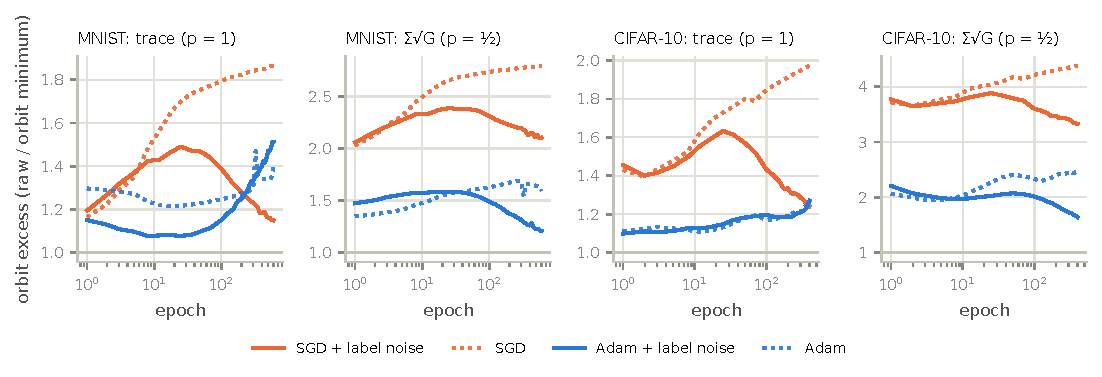
\includegraphics[width=0.92\textwidth]{fig7_labelnoise.pdf}
\caption{\textbf{Long horizons.} Orbit excess for the trace ($p=1$) and for $\sum_i\sqrt{G_{ii}}$ ($p=\tfrac12$) over 600 (MNIST) and 400 (CIFAR-10) epochs, with and without label noise (mean of two seeds). With label noise SGD moves toward the trace-minimizing point and Adam toward the $\sum_i\sqrt{G_{ii}}$-minimizing point.}
\label{fig:labelnoise}
\end{figure*}

SGD is not standing still on the orbit: its second-order term has expectation $\approx\frac{\eta^2}{B}(A_j-B_j)$ near a minimum, which pushes every unit toward curvature balance $A_j=B_j$, the stationarity condition of $\MS_1$ (the ``law of balance'' of \citealp{ziyin2023law}, written in curvature terms). The same argument in Adam's preconditioned coordinates predicts balance of $\sum\sqrt{G_{ii}}$, the stationarity condition of $\MS_{1/2}$. Ordinary training lives where Adam's fast first-order phase has acted and this slow phase has not.

Label noise \citep{blanc2020implicit,damian2021label} makes the slow phase visible. Over 600 (MNIST) and 400 (CIFAR-10) epochs (Fig.~\ref{fig:labelnoise}), Adam reaches an excess of $1.09$--$1.13$ within 5 epochs; without noise SGD's coordinates nearly stop moving once the data are fit; with noise SGD's trace excess falls steadily (CIFAR-10, $\eta=0.12$: $1.63\to1.24$), and Adam's $\sum\sqrt{G}$ excess falls ($1.99\to1.64$) while its trace excess \emph{rises} ($1.11\to1.27$). In every label-noise run SGD's trace excess falls more than its $\sum\sqrt{G}$ excess, and Adam's the other way round: 32 of 32 runs each, from 16 independent initializations (block-level sign test $p=3\times10^{-5}$); holding the curvature fixed and moving only along the orbit gives the same direction in 12 of 12 new runs each ($p=0.0005$). The predictions of \citet{damian2021label} and \citet{li2025adam} had so far been checked in diagonal linear networks and matrix factorization; the rescaling orbit provides a direction in a nonlinear network along which the predicted destination is known in closed form.

\textbf{Starting point.} Starting the \emph{same function} at three orbit points (first layer $\times\tfrac13,\times1,\times3$), the initial $7\times$ (MNIST) and $17\times$ (CIFAR-10) spread in excess collapses within one epoch for both optimizers: early curvature redistribution, not the starting coordinates, sets the excess. Adam nonetheless ends below SGD from every start ($1.09$--$1.35$ vs.\ $1.78$--$2.04$ on CIFAR-10; App.~\ref{sec:labelnoise-full}).

\subsection{Normalization layers}\label{sec:bn}
\begin{figure}[t]
\centering
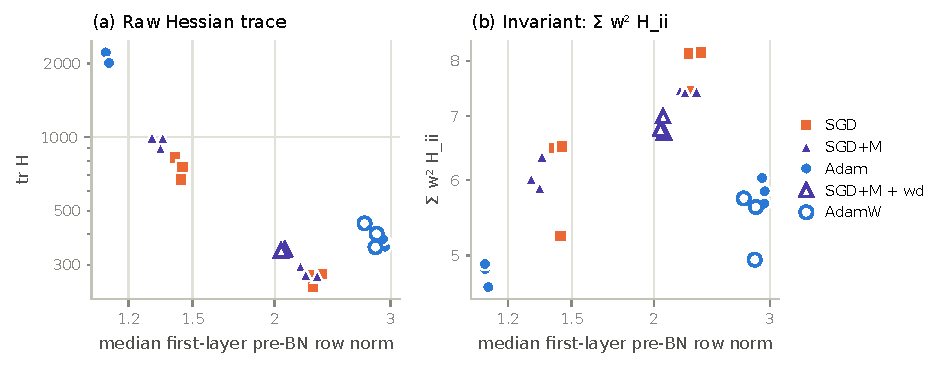
\includegraphics[width=\columnwidth]{fig8_bn.pdf}
\caption{\textbf{BatchNorm MLP} (CIFAR-10, training loss $0.1$; hollow: weight decay). \textbf{(a)} Raw trace follows the pre-BN weight norm, which the learning rate sets. \textbf{(b)} $\sum_iw_i^2H_{ii}$ does not, and ranks Adam lowest.}
\label{fig:bn}
\end{figure}

BatchNorm adds a second symmetry: the loss is invariant to scaling each pre-BN row, and every optimizer moves along it at a learning-rate-dependent rate \citep{vanlaarhoven2017l2,hoffer2018norm,arora2019autorate}. In a BatchNorm MLP on CIFAR-10 (24 runs), raw measures track the pre-BN norm (Spearman $-0.62$ to $-0.84$; Fig.~\ref{fig:bn}) and rate Adam \emph{sharper} than SGD ($P=0.25$), but their verdict flips with the learning-rate pairing (0/9 to 9/9 pairs). Measures invariant to every per-weight rescaling rate Adam \emph{flatter} in every pairing ($\sum_iw_i^2H_{ii}$: 70/72 pairs; ASAM: 72/72). In this MLP the coordinate factor thus reverses the ordering again, in the opposite direction.

\textbf{ResNet-18 on full CIFAR-10} (BatchNorm after every convolution; 24 GPU runs, three seeds; App.~\ref{app:extended}). Without augmentation or weight decay, the raw trace again follows the conv filter norms (Spearman $-0.62$ to $-0.96$), so its verdict is all or nothing per learning-rate pairing (Adam flatter in 22 of 54 seed-pairing-target triples), while $\sum_iw_i^2H_{ii}$ and ASAM rate Adam \emph{sharper} in 53 and 54 of 54. In the standard recipe (augmentation, weight decay, cosine schedule; 93--95\% test accuracy), the raw trace rates AdamW $1.3$--$4.9\times$ flatter than SGD+M in every seed, mostly through AdamW's $4$--$5\times$ larger filters, and the invariant measures do not confirm it (AdamW sharper in 7 of 9 pairs). Adam with coupled $L_2$ weight decay collapses many deep filters to zero \citep{mehta2019filter} and is excluded. Raw measures thus follow norms set by the learning rate and weight decay in both normalized networks, but the direction of the invariant verdict differs between them.

%===============================================================================
\section{Discussion and limitations}
%===============================================================================
\textbf{Recommendations.} Compare optimizers at matched training loss; report at least one rescaling-invariant measure (minimum sharpness is cheap given $\mathrm{diag}(G)$) or the orbit excess; state which invariant is used, since invariants can disagree (min-norm vs.\ minimum-trace point); do not rely on filter normalization; use SAM versus its base optimizer as a sanity check.

\textbf{Scope.} We do not claim that Adam's minima are universally sharper: invariant measures can disagree, sharpness depends on the learning rate, and invariant measures rate Adam flatter in a BatchNorm MLP but sharper in ResNet-18. We claim that raw-coordinate comparisons between Adam and SGD contain an optimizer-dependent coordinate factor with a precise mechanism, large enough to reverse conclusions in the settings tested. Only Proposition~\ref{prop:drift} and Lemma~\ref{lem:diag} are mathematical statements; the rest are measurements in the networks we trained. The generalization correlations are rank correlations in two MLP sweeps, not evidence that sharpness causes generalization. Our work is complementary to \citet{li2025adam}: they prove which sharpness Adam reduces near the minimizer manifold, while we study its fast drift along an exact symmetry and its effect on sharpness measurements. Most experiments use small networks on 10k-example subsets; the theory covers the ReLU rescaling symmetry; the explanation of where Adam's fast drift ends, and of its effect on Adam's noise floor, is heuristic.

\textbf{Conclusion.} A well-known caveat, that sharpness depends on the parameterization, has a systematic practical consequence: Adam breaks the rescaling conservation law that SGD obeys at first order and, in the networks we studied, holds its solutions near the flattest representation on their orbits. The resulting coordinate factor can reverse, flip or mask flatness rankings. Beyond measurement, the orbit separates a fast first-order drift of adaptive methods from a slow, noise-driven drift whose destination differs between SGD and Adam as implicit-regularization theory predicts.

\paragraph{Reproducibility.} All code, configurations and per-run results (training curves and every measure at every checkpoint) will be released.

\bibliographystyle{plainnat}
\bibliography{../refs}

\clearpage
\onecolumn
\appendix
% generated by build_appendix.py from ../main.tex -- do not edit by hand
\section{Extended results}\label{app:extended}
This appendix reproduces the complete results sections of the long version of this paper, with every number, control and caveat; figures and tables already shown in the main text are not repeated.

\subsection{Adam drifts along the orbit; SGD does not}\label{sec:mechanism-full}

We first isolate the mechanism. We log both terms of~\eqref{eq:decomp} at every step on the CIFAR-10 MLP, varying the learning rate ($3{\times}10^{-5}$--$10^{-3}$ for Adam, $0.01$--$0.1$ for SGD, $10^{-3}$--$10^{-2}$ for SGD+M) and the first layer's fan-in (inputs average-pooled to $8{\times}8$, $16{\times}16$ and $32{\times}32$), with two seeds per setting (66 runs). The decomposition closes to $\le1.3{\times}10^{-6}$ (float32 round-off) in every run.

\textbf{SGD conserves; Adam drifts.} SGD's first-order term is below $3{\times}10^{-7}$ in every run, zero up to round-off as Proposition~\ref{prop:drift}a requires. Adam's is $0.02$--$6.2$, five to seven orders of magnitude larger, and exceeds its own second-order term by $23$--$800\times$ (Fig.~\ref{fig:mechanism}a). SGD+M drifts only at second order, as Proposition~\ref{prop:drift}b predicts. At equal effective learning rate $\eta/(1-\beta)$ its total drift matches SGD's ($0.61$ vs.\ $0.58$ at $\eta_{\mathrm{eff}}=0.1$, $32{\times}32$).

\textbf{Scaling law.} A log-linear fit of Adam's first-layer first-order drift on $\log\eta$ and $\log\sqrt{d_{\mathrm{in}}}$ gives exponents $0.91$ and $0.94$ for $\eta\le10^{-4}$, close to the $\eta\sqrt{d_{\mathrm{in}}}$ predicted by Remark~\ref{rem:fanin} (Fig.~\ref{fig:mechanism}b). Over all learning rates the fit gives $1.07$ and $1.38$ ($R^2=0.97$). The steeper fan-in dependence at large $\eta$ is consistent with the remark, since the $\ell_1$ norms that drive the drift keep growing as training progresses further. The drift of the second layer, whose fan-in is fixed at 128, does not depend on input resolution. Seeds agree to within a few percent.

\textbf{Where the drift leads.} At initialization the CIFAR-10 MLP has orbit excess $E=3.66$; MNIST has $1.79$. During training, Adam moves to a median $E=1.11$--$1.28$ on CIFAR-10 and $1.21$--$1.24$ on MNIST, at every loss level (Fig.~\ref{fig:mechanism}c). Across all 90 Adam checkpoints, $E$ lies in $[1.08,1.48]$ on CIFAR-10, against $[1.45,4.89]$ for the other optimizers, and in $[1.12,1.48]$ on MNIST. As the $\eta$-proportional drift predicts, the excess is slightly higher at Adam's smaller base learning rate (CIFAR-10 median $1.29$--$1.38$ vs.\ $1.15$--$1.17$), where there is less drift to carry the network away from its initial coordinates. SGD cannot move along the orbit at first order, and SGD+M and SAM move along it only weakly (Proposition~\ref{prop:drift}b,d; in Table~\ref{tab:drift} their cumulative first-order terms are $0.069$ and $0.048$ at training losses $1.10$ and $0.90$, against $0.255$ for Adam at $1.13$), so their excess follows from their nearly conserved $Q_j$ combined with how the curvature redistributes during training; the second factor dominates, and SGD reaches a similar excess from very different starting points (\S\ref{sec:labelnoise}). Their median excess is $1.8$--$3.4$ on CIFAR-10 and drifts from $1.1$ to $1.6$ on MNIST. In parameter space, Adam's first-layer imbalance $|\log(\|a_j\|/\|c_j\|)|$ reaches $0.82$--$1.07$ on CIFAR-10 (an incoming/outgoing norm ratio of about $2.9$), compared with $0.30$--$0.46$ for the other optimizers, which stay near the initial $0.35$.

\textbf{Not specific to Adam.} Proposition~\ref{prop:drift}c covers every diagonal preconditioner. Repeating the drift experiment with RMSprop and with plain sign descent (signSGD, which has neither momentum nor second-moment estimates) gives the same picture (Table~\ref{tab:drift}). Both drift at first order, and with $32{\times}32$ inputs all three adaptive methods end at an orbit excess of $1.10$--$1.28$, against $1.68$--$2.41$ for SGD and SGD+M at comparable training losses. The common ingredient is that every coordinate takes a step of roughly the same size.

\paragraph{Where the drift leads: two phases.} The data and the theory point to two distinct phases.

\emph{Noise-driven phase (slow).} SGD is not standing still on the orbit. Its second-order term has expectation $\mathbb{E}D^{(2)}_j=\eta^2(\mathbb{E}\|g_{a_j}\|^2-\mathbb{E}\|g_{c_j}\|^2)$. Near a minimum, minibatch gradients are dominated by noise and the Fisher matrix approximates the Gauss--Newton matrix, so this is approximately $\frac{\eta^2}{B}(A_j-B_j)$. Here $A_j=\sum_{i\in\mathrm{in}(j)}G_{ii}$ and $B_j=\sum_{k\in\mathrm{out}(j)}G_{kk}$ are the unit's incoming and outgoing curvature. A positive drift enlarges the incoming weights, which lowers $A_j$ ($\propto c_j^{-2}$) and raises $B_j$ ($\propto c_j^{2}$). The drift therefore pushes every unit toward \emph{curvature balance} $A_j=B_j$, the stationarity condition of $\MS_1$. This is the ``law of balance'' of \citet{ziyin2023law,ziyin2024parameter} written in curvature terms, and the orbit component of the $\tr H$-minimizing implicit bias of label-noise SGD \citep{blanc2020implicit,damian2021label}; see also implicit gradient regularization \citep{barrett2021implicit}.

The same argument can be applied to Adam. For a quasi-static diagonal preconditioner $P$, Adam's update is an SGD step in the coordinates $\theta'=P^{1/2}\theta$. Because $P$ is diagonal it commutes with the rescaling, so Lemma~\ref{lem:euler} still holds in $\theta'$. The noise covariance in these coordinates is $P^{-1/2}\Sigma P^{-1/2}$. With $p_i\approx\sqrt{\mathbb{E}g_i^2}$, noise balance then requires $\sum_{\mathrm{in}}\sqrt{\Sigma_{ii}}=\sum_{\mathrm{out}}\sqrt{\Sigma_{kk}}$, i.e.\ $\sum_{\mathrm{in}}\sqrt{G_{ii}}=\sum_{\mathrm{out}}\sqrt{G_{kk}}$. That is the stationarity condition of $\MS_{1/2}$, the orbit restriction of the $\tr\,\mathrm{diag}(H)^{1/2}$ regularizer that \citet{li2025adam} derive rigorously for Adam. The heuristic therefore predicts \emph{different} long-run destinations: minimum trace for SGD and minimum $\sum_i\sqrt{G_{ii}}$ for Adam, both reached at $O(\eta^2)$ per step.

\emph{Signal-driven phase (fast).} Early in training the gradient has a large mean, and Adam's first-order term (Proposition~\ref{prop:drift}c) dominates. Empirically it takes Adam from an orbit excess of about $3.7$ at initialization to $\approx1.1$ within about five epochs on CIFAR-10 (\S\ref{sec:labelnoise}), i.e.\ close to the trace-minimizing point. We have only a heuristic for this destination. Adam's per-coordinate steps have roughly equal size $\eta$ whatever the curvature, so the loss injected by its update noise, $\approx\frac{\eta^2}{2}\sum_iH_{ii}r_i^2$ with $r_i$ roughly constant, is proportional to $\tr H$ in the current coordinates. SGD has no first-order drift, so in this phase it stays wherever its initialization and its conserved $Q_j$ put it.

Ordinary training, and every optimizer comparison in \S\ref{sec:audit}, lives in the regime where the fast phase has acted and the slow phase has not. \S\ref{sec:labelnoise} tests both phases directly.

\subsection{Consequence: the coordinate factor reverses optimizer rankings}\label{sec:audit-full}

\paragraph{CIFAR-10.} Figure~\ref{fig:flip} and Table~\ref{tab:flip} summarize the audit. At every matched training loss, Adam is rated flatter than SGD by the original metric ($P=0.62$--$0.67$), isotropic average sharpness ($0.69$--$0.75$), the Hessian trace ($0.62$--$0.74$) and, most strongly, $\sum_i\sqrt{G_{ii}}$ ($0.84$--$1.00$). Minimum sharpness reverses the conclusion ($P=0.01$--$0.22$), as do $\MS_{1/2}$ ($0.01$--$0.19$), filter-normalized sharpness ($0.06$--$0.14$), multiplicative sharpness ($0.16$--$0.31$) and $\sum w_i^2G_{ii}$ ($0.04$--$0.24$). With 18 runs per optimizer the raw verdicts carry substantial uncertainty (e.g.\ $\tr G$ at loss $0.1$: $P=0.64$, 95\% CI $[0.44,0.83]$), whereas the invariant verdicts are tight ($\MS_1$: $0.01$, $[0.00,0.06]$). The quantity that matters, the disagreement between them, is well determined: $P_{\tr G}-P_{\MS_1}=+0.69$ $[+0.52,+0.83]$, $+0.63$ $[+0.43,+0.81]$ and $+0.50$ $[+0.34,+0.67]$ at losses $0.3$, $0.1$ and $0.01$. The exact split explains this. In bits, $\log_2(\tr G_{\mathrm{Adam}}/\tr G_{\mathrm{SGD}})$ decomposes into a function term of $+0.52$ $[+0.36,+0.68]$, $+0.71$ $[+0.53,+0.87]$ and $+0.43$ $[+0.16,+0.71]$ (Adam sharper), and a coordinate term of $-1.03$ $[-1.17,-0.91]$, $-1.02$ $[-1.16,-0.87]$ and $-1.05$ $[-1.22,-0.89]$, a factor of almost exactly $2$ in Adam's favour at every loss level. Against SGD+M the coordinate term is larger still ($-0.94$ to $-1.33$ bits). Against SAM, the one optimizer designed to seek flat minima, the raw trace is inconclusive ($P=0.44$--$0.60$) because a large function term ($+0.69$ to $+1.00$ bits, SAM flatter) is cancelled by the coordinate term ($-0.69$ to $-0.92$). Invariant measures identify SAM as clearly flatter ($P=0.00$--$0.23$). A measure that fails this sanity check should not be used to rank optimizers.

\textbf{Robustness to the learning-rate pairing.} Sharpness depends strongly on the learning rate, so we also split the comparison by the pair of base learning rates (Table~\ref{tab:lrpairs}, pooled over batch sizes, seeds and losses $0.1$--$0.01$). On CIFAR-10 the raw verdict is set by the pairing: $P$ for $\tr G$ is $1.00$, $0.06$, $1.00$ and $0.60$ in the four pairings, and the original metric ranges from $0.00$ to $1.00$. Minimum sharpness rates Adam sharper in all four pairings ($P\le0.27$), and so does filter-normalized sharpness ($P\le0.09$). On MNIST both raw and invariant verdicts depend on the pairing ($\MS_1$: $0.00$--$0.88$), consistent with the small functional differences there.

\paragraph{MNIST.} Here the initial excess is smaller and the picture shifts during training (Fig.~\ref{fig:flip}b). Early on (training loss $1$ to $0.3$), SGD's excess is \emph{below} Adam's. The coordinate term therefore slightly favours SGD ($+0.15$ $[+0.12,+0.19]$ bits at loss $0.3$), and raw measures rate Adam sharper ($P=0.06$ for the trace). As SGD's excess grows, the coordinate term turns in Adam's favour ($-0.40$ $[-0.41,-0.38]$ bits at loss $0.01$) and the raw trace ordering flips ($P=0.80$, $[0.63,0.94]$). The original metric goes from $0.27$ to $0.97$. The function term never favours Adam: it shrinks from $+0.34$ to $+0.04$ bits (the latter indistinguishable from zero, $[-0.13,+0.22]$), and minimum sharpness gives $P=0.09$, $0.28$ and $0.44$ at losses $0.3$, $0.1$ and $0.01$. On MNIST, then, whether ``Adam is flatter'' depends on \emph{when} one measures, and the dependence comes almost entirely from the coordinate factor.

\paragraph{Invariant measures need not agree with each other.} Invariance removes the coordinate artifact, but it does not make different notions of flatness coincide. On CIFAR-10 all invariant measures agree, with one exception: large-radius ASAM at the earliest target ($P=0.71$ at loss $0.3$, then $0.32$ and $0.28$). On MNIST, the elementwise-relative family (multiplicative sharpness, ASAM, $\sum_iw_i^2G_{ii}$) rates Adam flatter late in training ($P=0.73$--$0.87$ at loss $0.01$), while minimum sharpness and filter-normalized sharpness do not ($0.44$ and $0.20$). The relative measures weight each weight's curvature by its squared magnitude, which is itself affected by Adam's sign-like updates. We therefore make no universal claim that Adam's minima \emph{are} sharper. Our claim is narrower and robust: the raw-coordinate ordering is biased by an optimizer-dependent factor that is as large as the effects being measured.

\paragraph{$\lambda_{\max}$ and canonicalization.} The top eigenvalue rates Adam sharper even in raw coordinates ($P=0.29$--$0.45$ on CIFAR-10, $0.00$--$0.32$ on MNIST), in line with prior reports and with edge-of-stability dynamics. It is dominated by a few outlier directions, while the drift mainly reshapes the bulk of the diagonal that trace-type and isotropic measures integrate. Mapping each network to its minimum-norm representative before measuring only partly removes the bias ($P=0.31$--$0.56$ for the trace on CIFAR-10). Adam's drift moves toward \emph{curvature} balance, which is the condition for minimum sharpness, not toward norm balance.


\subsection{Causal test: removing Adam's drift}\label{sec:intervention-full}

If the coordinate factor is caused by Adam's drift, removing the drift should change raw measures and leave invariant ones alone. \emph{Adam-Q} runs Adam and, after every step, applies the function-preserving rescaling that restores each unit's $Q_j$ to its initial value. For a single unit this requires solving $c^2\|a_j\|^2-\|c_j\|^2/c^2=Q^{(0)}_j$ for $c>0$, which has a closed form. Because rescaling a unit also changes the incoming weights of the next layer, we apply these per-unit solutions layer by layer in two sweeps. The restoration is therefore approximate: in a check over 300 Adam steps on the CIFAR-10 MLP (inspected at steps 1, 100 and 300), the remaining deviation of $Q_j$ from $Q^{(0)}_j$ was at most $7\times10^{-4}$ of $\max_j|Q^{(0)}_j|$ in the first layer and $3\times10^{-7}$ in the second, did not accumulate, and the network output changed by at most $4\times10^{-6}$ per restoration. Adam's moment estimates are transformed covariantly: for a weight scaled by $s$, $m\mapsto m/s$ and $v\mapsto v/s^2$. Since the rescaling preserves the function, Adam-Q optimizes the same loss and differs from Adam only through Adam's lack of rescaling-equivariance. We rerun the 18 Adam configurations of each main sweep with Adam-Q and compare checkpoints of the same configuration whose training losses agree to within $25\%$ (73 of 78 pairs on CIFAR-10).

In 12 of the 18 CIFAR-10 configurations (base learning rate $10^{-4}$, and all runs at batch size 512) Adam-Q trains like Adam, reaching every loss target in the same or slightly fewer epochs. In the six noisiest configurations (base rate $3\times10^{-4}$ at batch sizes 32 and 128), however, Adam-Q stalls. It reaches loss $0.1$ two to three times later than Adam and never gets below $\approx0.05$ within 300 epochs, whereas Adam reaches $0.01$ by epoch $\approx55$. On MNIST all 18 Adam-Q runs train normally. So the drift is not merely a measurement nuisance: in noisy regimes it appears to help Adam train. Three controls, each run with two seeds at the three base settings, narrow this down. First, restoring $Q_j$ only every 50 steps instead of every step still stalls at batch sizes 32 and 128, so the stall is not caused by intervening at every step. Second, restoring $Q_j$ in only one hidden layer trains normally. Freezing just the first layer, which has fan-in 3072 and the largest drift, reaches loss $0.01$ in 57--78 epochs; freezing just the second takes 52--62, against 52--67 for Adam. The obvious hypothesis, that Adam must inflate its high-fan-in weights to shrink their relative step $\eta/|w_i|$, is therefore wrong: the stall appears only when both layers are prevented from drifting. Third, restoring $Q_j$ \emph{without} transforming Adam's moment estimates stalls at every batch size, including 512. That version is a harsher intervention rather than a cleaner control, which is why the covariant transformation is part of Adam-Q.

\textbf{Where Adam is held, not whether it is held, causes the stall.} A fourth control separates the intervention from the orbit position. Every 100 steps we move Adam, with its moment estimates transformed covariantly, to a chosen point of its current orbit and let it drift freely in between: either to the minimum-trace point, or to the minimum-norm point, which is where Adam-Q ends up (its imbalance falls to $0.02$). We use the same three settings and two seeds (12 runs). Held at the minimum-trace point (orbit excess $1.00$--$1.01$ at every checkpoint), Adam trains as fast as unconstrained Adam: all six runs reach loss $0.01$, in 51--61 epochs against 52--67. Held at the minimum-norm point (excess $2.1$--$2.8$ from loss $0.3$ on), all four runs at batch sizes 32 and 128 stall like Adam-Q, at a final loss of $0.17$--$0.30$ after 300 epochs (Adam-Q: $0.18$--$0.30$), while the two runs at batch size 512 still reach $0.01$. The intervention itself is therefore harmless, and what slows Adam is being kept at coordinates with a large orbit excess. This is what the heuristic of \S\ref{sec:mechanism} predicts: Adam's per-coordinate steps have roughly equal size, so the loss its update noise injects scales with the trace in its \emph{current} coordinates, about $2\times$ larger at the minimum-norm point than near the minimum-trace point, and the difference matters only when the gradient noise is large. Adam's drift toward the minimum-trace point thus lowers its own noise floor; it helps Adam train as well as making its minima look flat. All comparisons below use only checkpoint pairs that are genuinely loss-matched. Across them, test accuracy at matched loss differs by a median factor of $0.995$. Adam-Q's coordinates stay SGD-like: first-layer imbalance falls from $0.89$ to $0.13$ and the orbit excess rises from $1.18$ to $2.35$. Figure~\ref{fig:intervention} shows the consequence on CIFAR-10. Every raw trace-type measure roughly doubles: $\tr G$ by a median factor of $1.91$ (IQR $1.63$--$2.04$), the isotropic average by $1.96$ and the original metric by $1.64$. The invariant measures are essentially unchanged: $\MS_1$ $0.98$ (IQR $0.94$--$1.03$), $\MS_{1/2}$ $0.99$, multiplicative $1.09$, and the partially invariant filter-normalized measure $0.99$. $\lambda_{\max}$ moves less ($1.23$, IQR $0.94$--$1.49$), consistent with its weaker dependence on the coordinate factor (\S\ref{sec:audit}). Ranked against SGD, Adam-Q is no longer rated flatter: $P(\text{flatter than SGD})$ by $\tr G$ drops from $0.64$--$0.75$ (Adam) to $0.21$--$0.35$ (Adam-Q), and by the original metric from $0.62$--$0.67$ to $0.12$--$0.34$. Minimum sharpness gives the same verdict for both ($0.06/0.01/0.22$ vs.\ $0.00/0.02/0.21$ at losses $0.3/0.1/0.01$; at $0.01$ only the 12 Adam-Q configurations that reach it are included). The one deviation is at the lowest loss target ($0.01$), where the median $\MS_1$ ratio is $0.88$. There, small residual differences between the two trajectories matter because cross-entropy curvature scales with the loss.

On MNIST the intervention changes little, which is what the decomposition predicts. MNIST's conserved coordinates happen to lie close to the orbit minimum (initial excess $1.79$ vs.\ $3.66$ on CIFAR-10), so Adam-Q's excess ($1.11$--$1.36$ across loss targets, median $1.17$) stays near Adam's ($1.21$). The raw measures accordingly move by at most about $13\%$ (median $\tr G$ ratio $0.88$--$1.07$ across targets), and the invariant measures are again unchanged ($\MS_1$ $0.99$, IQR $0.98$--$1.00$; $\MS_{1/2}$ $0.99$). Together the two datasets give a dose--response: Adam-Q moves raw sharpness in proportion to how far it moves the coordinates ($\times1.9$ when the excess doubles on CIFAR-10, about $\pm10\%$ when it barely changes on MNIST), and moves minimum sharpness in neither case. Only $\lambda_{\max}$ behaves differently on MNIST ($\times0.82$), a reminder that it is not rescaling-invariant either.

\textbf{What the intervention does and does not show.} Each Adam-Q rescaling preserves the network output to float32 precision ($3\times10^{-6}$, Appendix~\ref{app:measures}), uses the same loss, minibatches, learning rate and schedule as Adam, and transforms the optimizer state covariantly. It does \emph{not} leave the later trajectory unchanged: because Adam is not rescaling-equivariant, every subsequent step differs, which is how the stall arises. We therefore compare only checkpoint pairs that are matched in training loss, never runs at equal epochs. Part of the result is also arithmetic: since $\tr G=\MS_1\times E$ exactly, doubling $E$ doubles the trace unless $\MS_1$ changes. The empirical content is that it does not change ($\times0.98$): at matched loss, the drift changes where Adam sits on the orbit but not, measurably, the function-level sharpness or test accuracy of what it finds. Removing Adam's flatness advantage over SGD is the consequence of that. The intervention establishes that Adam's drift causes the coordinate factor in these MLPs; it does not, on its own, establish anything about why Adam generalizes as it does.

\subsection{Are Adam's coordinates good coordinates for SGD?}\label{sec:teleport-full}
If Adam ends near the trace-minimizing point and SGD does not, would SGD benefit from being moved there? Symmetry teleportation makes this cheap to test \citep{zhao2022teleport,zhao2024improving}, since our target has a closed form. Every 100 steps we map SGD (or SGD+M) to the minimum-sharpness point of its current orbit, computed from $\mathrm{diag}(G)$ on 1024 training examples, and transform the momentum buffer covariantly. We use four learning rates per optimizer and two seeds on the CIFAR-10 MLP.

It does not help; it destabilizes training. Ten of the 16 teleported runs diverged, against none of the 16 plain runs. At $\eta=0.12$, for instance, plain SGD reaches loss $0.01$ in 52--53 epochs, while both teleported runs diverge. The two teleported runs that did reach loss $0.01$ generalized worse (test accuracy $0.392$--$0.396$ vs.\ $0.433$--$0.441$).

The reason is the top eigenvalue. Logging $\lambda_{\max}$ around every teleport of an $\eta=0.12$ run, each teleport \emph{raised} it by 3--20\%, leaving it within 5\% of, or above, SGD's stability threshold $2/\eta=16.7$ in 8 of 11 teleports. SGD on its own keeps $\lambda_{\max}$ just below $2/\eta$, the self-stabilization of gradient descent at the edge of stability \citep{cohen2021eos,damian2023selfstabilization}, and the teleports keep knocking it over. The teleport scales were mild ($0.95$--$2.5$), so this is not an artifact of extreme rescalings. Measured on the converged networks, the same map \emph{lowers} $\lambda_{\max}$ (e.g.\ $15.9\to11.0$), so the trace and the top eigenvalue are minimized at different points of the orbit, and which point is ``better'' depends on what the optimizer needs. Adam's preferred coordinates are good for Adam, not for SGD.

\subsection{Long horizons: the orbit as a testbed for implicit sharpness regularization}\label{sec:labelnoise-full}

The two-phase picture makes predictions that ordinary training cannot test, because the slow phase needs persistent gradient noise and long horizons. Implicit-regularization theory supplies the standard device for this: \emph{label noise}, in which every label is replaced by a uniformly random class with probability $0.2$, freshly at every step \citep{blanc2020implicit,damian2021label}. We train the MLPs for 600 (MNIST) and 400 (CIFAR-10) epochs with SGD ($\eta\in\{0.06,0.12\}$) and Adam ($\eta\in\{2,6\}\times10^{-4}$), with and without label noise, two seeds each (32 runs), and track the orbit excess for $p=1$ and $p=\tfrac12$ (Fig.~\ref{fig:labelnoise}). Both targets are computable exactly. To our knowledge, the predictions of \citet{damian2021label} and \citet{li2025adam} had so far been checked only in diagonal linear networks and matrix factorization. The rescaling orbit gives a direction in a nonlinear network along which the predicted destination is known in closed form.

\textbf{Fast phase.} From an orbit excess of about $3.7$ at initialization, Adam reaches $1.09$--$1.13$ by epoch 5 on CIFAR-10 in all four Adam settings, while SGD is at $1.45$--$1.63$.

\textbf{Without noise, SGD freezes.} SGD's excess rises while the data are being fit and then stops changing once gradients vanish ($1.78$--$1.86$ on MNIST, $1.97$--$2.67$ on CIFAR-10).

\textbf{With label noise, SGD moves toward minimum trace.} After the initial transient its trace excess falls steadily: on CIFAR-10 from $2.05$ (epoch 25) to $1.63$ at $\eta=0.06$, and from $1.63$ to $1.24$ at $\eta=0.12$; on MNIST from $1.65$ (epoch 100) to $1.35$, and from $1.39$ to $1.15$. The movement is faster at the larger learning rate, as a second-order drift should be. Its per-unit curvature balance at $p=1$ shrinks markedly (CIFAR-10, $\eta=0.12$: mean $|\log A_j/B_j|$ from $1.37$ to $0.80$), while balance at $p=\tfrac12$ barely changes ($2.31$ to $2.04$).

\textbf{With label noise, Adam moves toward minimum $\sum_i\sqrt{G_{ii}}$.} At $\eta=6\times10^{-4}$, Adam's $p=\tfrac12$ excess falls (MNIST $1.56\to1.21$, CIFAR-10 $1.99\to1.64$) while its trace excess \emph{rises} (MNIST $1.10\to1.51$, CIFAR-10 $1.11\to1.27$).

\textbf{A per-run test.} For each run we compare the change in log excess from epoch 100 to the end at $p=\tfrac12$ with that at $p=1$. In all 8 label-noise SGD runs the trace excess falls by more (mean difference $+0.090$), and in all 8 label-noise Adam runs the $\sum\sqrt{G}$ excess falls by more (mean $-0.219$); a two-sided sign test gives $p=0.008$ for each. Each optimizer thus drifts toward the orbit point favoured by its own implicit regularizer. The ordinary-training regime of \S\ref{sec:audit} corresponds to the end of the fast phase, before this slow drift has had time to act.

\begin{figure}[t]
\centering
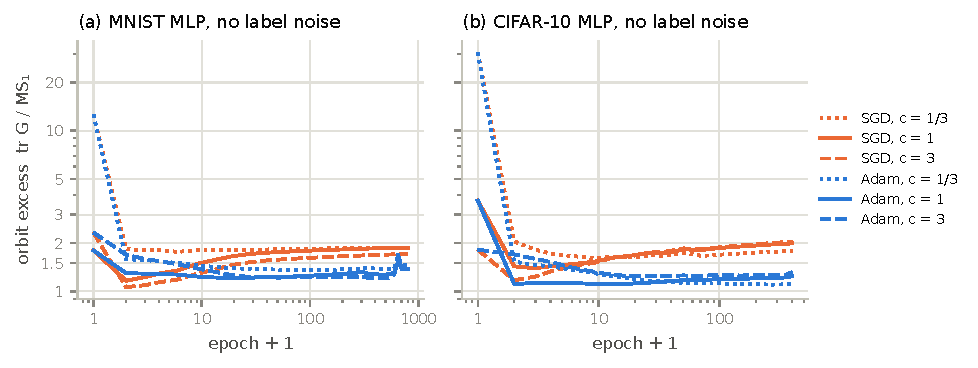
\includegraphics[width=0.9\linewidth]{fig9_memory.pdf}
\caption{\textbf{Coordinate memory.} The same initial function started at three points of its orbit (first-layer weights $\times c$, second layer $\div c$), trained without label noise (mean of two seeds). The initial spread in orbit excess disappears within one epoch for both optimizers, but from every starting point Adam ends below SGD.}
\label{fig:memory}
\end{figure}

\textbf{Does the starting orbit point matter?} Our account of SGD's excess leans on its conservation law, so we tested it directly. We start the \emph{same initial function} at three points of its orbit, multiplying the first layer's incoming weights and biases by $c\in\{\tfrac13,1,3\}$ and dividing the second layer's weights by $c$, and train with SGD and Adam, with and without label noise, for 800 (MNIST) and 400 (CIFAR-10) epochs (same learning rates as above, two seeds; 48 runs). The initial excess differs by a factor of $7.0$ (MNIST) and $16.9$ (CIFAR-10) across $c$ (Fig.~\ref{fig:memory}).\footnote{The CIFAR-10 runs of this experiment were done on a machine that could not reach the original CIFAR-10 host. We used a lossless PNG copy, whose ordering differs, so their 10k training subset differs from that of the other CIFAR-10 experiments.}

The prediction that SGD would remember its starting point in the orbit excess fails, and the reason is informative. For every optimizer, the spread across $c$ collapses to $1.3$--$1.9\times$ within the first epoch and ends at $1.03$--$1.19\times$ (one exception: $1.38\times$ for Adam with label noise on CIFAR-10). The curvature redistribution of early training, not the starting coordinates, sets the excess. SGD does remember its starting point in \emph{parameter} space: without label noise it keeps $90$--$99\%$ of the initial separation in mean first-layer $Q_j$ between $c=3$ and $c=\tfrac13$, and with label noise $79$--$83\%$. Adam does not erase that separation either. It enlarges it, to $1.5$--$2.0\times$ in seven of eight runs (and $0.97\times$ in one), consistent with a drift proportional to the units' $\ell_1$ norms (Remark~\ref{rem:fanin}). What does not depend on the starting point is the gap between the optimizers. Without label noise Adam ends at an excess of $1.29$--$1.51$ on MNIST and $1.09$--$1.35$ on CIFAR-10 from every starting point, against $1.71$--$1.89$ and $1.78$--$2.04$ for SGD. Starting SGD at a low excess does not keep it there (CIFAR-10, $c=3$: $1.82\to2.03$). Adam's low excess is therefore not an accident of the default initialization, and SGD's higher excess is where its own dynamics lead from any of these starting points.

The slow phase replicates across starting points. In the per-run test above (epoch 100 to the end), SGD's trace excess falls by more than its $\sum_i\sqrt{G_{ii}}$ excess in all 12 label-noise runs, and Adam's $\sum_i\sqrt{G_{ii}}$ excess falls by more in all 12 (sign test $p=0.0005$ each).

\textbf{Per-unit drift direction.} Between consecutive snapshots we correlate each hidden unit's change in $Q_j$ with its curvature imbalance $\log(A_j/B_j)$ at $p=1$ and at $p=\tfrac12$ (Spearman over units, averaged over snapshot pairs). Drift toward balance at power $p$ predicts a positive correlation at that $p$. Adam's per-unit drift matches $p=\tfrac12$ better than $p=1$ in every run, window and setting (24 of 24 runs, early and late). With label noise, the late-phase correlation is $+0.49$ at $p=\tfrac12$ against $-0.06$ at $p=1$ on MNIST, and $+0.18$ against $-0.16$ on CIFAR-10. Without label noise Adam's units drift \emph{away} from trace balance ($-0.25$ and $-0.56$; negative in 12 of 12 runs), as expected if the first-order sign-descent term rather than curvature dominates. For SGD the unit-level picture is mixed. On MNIST with label noise the drift matches $p=1$ better ($+0.39$ vs.\ $+0.26$, 6 of 6 runs). On CIFAR-10 it correlates positively with both but more strongly with $p=\tfrac12$ ($+0.60$ vs.\ $+0.76$, 0 of 6 runs favour $p=1$), although at the orbit level the same runs move toward minimum trace. The Fisher $\approx$ Gauss--Newton step of our heuristic is the likely weak point here. We therefore regard the orbit-level destinations, which replicate in 40 of 40 label-noise runs across both experiments, as established, and the unit-level mechanism for SGD as only partly confirmed.

\subsection{Consequences for generalization prediction}\label{sec:generalization-full}

If the coordinate factor is a \emph{cross-optimizer} bias, it should hurt generalization prediction mainly when models from different optimizers are ranked together. This is what we find (Fig.~\ref{fig:gen}). Within one optimizer, raw $\tr G$ and $\MS_1$ predict the accuracy gap equally well (mean Kendall $\tau$ at loss $0.01$: $0.55$ vs.\ $0.59$ on CIFAR-10, $0.54$ vs.\ $0.54$ on MNIST). Pooled across optimizers, $\tr G$ drops to $0.38$ (CIFAR-10) and $0.47$ (MNIST), while $\MS_1$ stays at $0.61$ and $0.62$. The gain from removing the coordinate factor is larger on CIFAR-10 ($+0.21$ to $+0.23$ across loss targets) than on MNIST ($+0.01$ to $+0.15$), matching the smaller coordinate term there. A bootstrap over runs (stratified by optimizer, 2000 resamples) gives a pooled improvement from $\tr G$ to $\MS_1$ at loss $0.01$ of $+0.24$, 95\% CI $[+0.14,+0.33]$, on CIFAR-10 and $+0.15$ $[+0.09,+0.20]$ on MNIST. The original metric is the weakest cross-optimizer predictor ($0.36$ on CIFAR-10, $0.14$ on MNIST). Not every raw measure behaves like the trace: $\lambda_{\max}$ and worst-case SAM sharpness, which depend less on the coordinate factor, reach a pooled $\tau$ of $0.49$--$0.61$ on CIFAR-10 without any correction. We use the accuracy gap rather than the test loss as the target. This choice was made after seeing the test-loss correlations: at matched training loss in this memorization regime, the test loss is dominated by over-confident errors, and on CIFAR-10 it is negatively correlated with most measures (pooled $\tau$ between $-0.46$ and $+0.07$ at loss $0.01$ for all 17; \texttt{scripts/gen\_correlation.py} prints both tables). These are rank correlations over the configurations of two MLP sweeps. They show that the coordinate factor degrades cross-optimizer comparisons here; they do not show that invariant sharpness is a better predictor of generalization in general, or that sharpness causes generalization.

\subsection{Revisiting the original study}\label{sec:replication-full}

Table~\ref{tab:replication} re-runs the original fixed-epoch protocol with five seeds. The original result replicates: the relative perturbation metric is about $2.9\times$ lower for Adam on both datasets. The two datasets fail for different reasons, however. On \textbf{CIFAR-10}, both optimizers are far from convergence at similar training losses ($1.29$ vs.\ $1.42$). The $2.5\times$ gap in Hessian trace is almost entirely the coordinate factor ($E=1.23$ vs.\ $2.85$, i.e.\ $2.3\times$), the minimum sharpness is nearly equal ($320$ vs.\ $353$), and the invariant multiplicative measure and the partially invariant filter-normalized measure rate Adam about $2.5\times$ \emph{sharper}. On \textbf{MNIST}, after 20 epochs Adam has reached a $17\times$ lower training loss than SGD ($0.008$ vs.\ $0.136$), and every measure, invariant or not, is correspondingly lower. That is a loss-level confound of fixed-epoch comparisons, not a property of the optimizer, and matching the loss removes it (\S\ref{sec:audit}). One further detail of the original study may also have contributed. Its single Adam run on CIFAR-10 reported only $33.7\%$ test accuracy, against $49.6\pm0.5\%$ in our five-seed PyTorch replication. The difference may come from framework defaults (Keras uses Glorot initialization and $\epsilon=10^{-7}$) or from an unstable run. In our pilot runs with raw, uncentred inputs, Adam at $\eta=10^{-3}$ could oscillate around a training loss of $\approx1$. Either way, a high final loss lowers the relative metric $\Delta L/L$ mechanically.

\subsection{Convolutional networks}\label{sec:cnn-full}

We repeat the audit on the CNN with SGD, SGD+M and Adam (two learning rates each, batch size 128, three seeds; 18 runs). Rescaling now acts on whole channels, and minimum sharpness is computed from the exact per-sample $\mathrm{diag}(G)$ on 512 examples. Fifteen runs reached every loss target. The three Adam runs at the lower learning rate ($10^{-4}$) reached training loss $0.018$--$0.034$ by the 150-epoch cap, so comparisons at loss $0.01$ use only the other three Adam runs.

The mechanism carries over (Fig.~\ref{fig:cnn}a). Adam's channel imbalance is roughly twice SGD's in all three hidden layers (median $0.53/0.55/1.47$ vs.\ $0.22/0.35/0.65$ at loss $0.1$). Its orbit excess stays low at every loss level (median $1.45$, $1.78$, $1.68$ at losses $1$, $0.1$, $0.01$), while SGD's and SGD+M's grow from $1.7$--$1.8$ to $3.2$. The coordinate term again favours Adam and grows during training: $-0.31$ $[-0.38,-0.23]$, $-0.71$ $[-0.91,-0.49]$ and $-0.93$ $[-1.06,-0.79]$ bits against SGD, and $-0.24$ to $-0.91$ bits against SGD+M.

On this network, however, Adam's solutions are clearly sharper at the function level ($+1.27$ to $+2.30$ bits against SGD, $+0.68$ to $+1.24$ against SGD+M; all intervals exclude zero), and every invariant measure rates Adam sharper than both baselines ($P=0.00$ at every loss for $\MS_1$, multiplicative and $\sum_iw_i^2G_{ii}$), and so does the partially invariant filter-normalized measure. The coordinate factor therefore does not reverse the ranking here. It \emph{hides} part of the difference. Against SGD+M it hides most of it: the raw trace ratio is $+0.44$, $+0.57$ and $+0.18$ bits with intervals that include zero, and raw measures are inconclusive ($P=0.25$--$0.50$ for the trace and the original metric). A researcher using raw measures would conclude that Adam and SGD+M find equally flat minima on this CNN; an invariant measure shows Adam's are about $2\times$ sharper. Across the three settings, the same coordinate bias in Adam's favour thus reverses the ranking (CIFAR-10 MLP), flips it during training (MNIST MLP), or masks a large functional difference (CIFAR-10 CNN), depending on how large the functional difference is.


\subsection{Depth}\label{sec:depth-full}

Does the coordinate factor compound with depth, since every hidden layer adds its own rescaling symmetry? We train CIFAR-10 MLPs with $L\in\{1,2,4,8\}$ hidden layers of width 128 with SGD ($\eta=0.06$), SGD+M ($0.006$) and Adam ($6\times10^{-4}$), batch size 128 and three seeds (36 runs). All use He initialization with zero biases so that the signal is preserved at every depth, and all reached the targets $1$, $0.3$ and $0.1$.\footnote{These runs use the reordered CIFAR-10 copy described in \S\ref{sec:labelnoise}.} The answer is no (Fig.~\ref{fig:depth}). Adam's orbit excess stays at $1.16$--$1.39$ and SGD's and SGD+M's at $1.50$--$2.15$ at every depth. The coordinate term against SGD is $-0.48$ to $-0.74$ bits at every depth and target except the earliest target at depth 1 ($-0.15$), and against SGD+M it is $-0.47$ to $-0.88$ bits (again except the earliest target at depth 1, $-0.25$), a factor of $1.4$--$1.8$ in Adam's favour. What grows with depth is the function term: against SGD it rises from $+0.26$--$+0.37$ bits at depth 1 to $+0.76$--$+0.89$ at depth 8, and minimum sharpness rates Adam sharper than SGD in every pair at every depth ($P=0.00$). The consequence mirrors \S\ref{sec:audit} and \S\ref{sec:cnn-full} within one architecture family. At depths 1 and 2 the raw trace rates Adam flatter than SGD in every pair at losses $0.3$ and $0.1$ ($P=1.00$) while minimum sharpness rates it sharper in every pair ($P=0.00$): the ordering reverses. At depth 8 the raw trace rates Adam sharper as well, but by $+0.23$ to $+0.37$ bits instead of the $+0.84$ to $+0.89$ bits of the function term, so the coordinate factor hides most of the difference.

\subsection{Normalization layers and weight decay}\label{sec:bn-full}

BatchNorm adds a second symmetry. The loss is invariant to scaling each row of a pre-BN weight matrix, so the curvature with respect to that row scales as $1/\|w_{\mathrm{row}}\|^2$, and every optimizer moves along this symmetry: the gradient is orthogonal to a scale-invariant row, so even SGD grows its norm at second order, at a rate set by the learning rate \citep{vanlaarhoven2017l2,hoffer2018norm,arora2019autorate}. The ReLU rescaling survives between the BN affine parameters and the next layer. We test whether the coordinate factor still matters with the MLP of \S\ref{sec:protocol} with BatchNorm after each hidden linear layer (no bias before BN), trained on CIFAR-10 with SGD ($\eta\in\{0.1,0.3\}$), SGD+M ($\{0.01,0.03\}$), Adam ($\{3,10\}\times10^{-4}$), SGD+M with weight decay $5\times10^{-4}$ ($\eta=0.03$) and AdamW (weight decay $0.05$, $\eta=10^{-3}$), batch size 128 and three seeds (24 runs). All runs reached the targets $1$, $0.3$ and $0.1$, the last after a median of 35--44 epochs, and all are within $0.42$--$0.45$ test accuracy. The orbit-minimum machinery does not apply (BN couples the samples), so we compare raw measures with the measures that are invariant to every per-weight rescaling: $\sum_iw_i^2H_{ii}$ (Hutchinson), multiplicative average sharpness and ASAM. All measures use batch statistics.

\textbf{Raw measures read off the weight norm} (Fig.~\ref{fig:bn}). Across the 24 runs, the Hessian trace, $\lambda_{\max}$ and isotropic sharpness are strongly anticorrelated with the median first-layer pre-BN row norm (Spearman $\rho=-0.84$, $-0.76$, $-0.62$ for the trace at losses $1$, $0.3$, $0.1$). The invariant measures are not ($\rho$ between $-0.30$ and $+0.23$ for $\sum_iw_i^2H_{ii}$ and ASAM). The norms are set mostly by the learning rate. At loss $0.1$ the median first-layer row norm is $1.1$ for Adam at $3\times10^{-4}$ and $2.9$ at $10^{-3}$, against $1.3$--$1.4$ for SGD and SGD+M at their smaller rates and $2.2$--$2.3$ at their larger ones. Adam keeps its second-layer rows short at both rates ($0.61$ and $0.84$, against $0.95$--$1.71$ for SGD and SGD+M).

\textbf{The raw verdict depends on the learning-rate pairing; the invariant verdict does not.} Pooled over pairings, raw measures rate Adam \emph{sharper} than SGD ($P=0.25$ at every target for the trace, $\lambda_{\max}$ and isotropic sharpness; trace ratio $+0.38$, $+0.84$, $+1.00$ bits). Split by pairing, however, Adam at $3\times10^{-4}$ is rated flatter by the trace in $0$ of $9$ seed-and-target pairs against each of the four SGD and SGD+M settings, while Adam at $10^{-3}$ is rated flatter in $9/9$ against SGD at $\eta=0.1$ and SGD+M at $0.01$, in $4/9$ against SGD+M at $0.03$, and in $0/9$ against SGD at $0.3$ (22 of 72 pairs overall). The invariant measures rate Adam \emph{flatter} in every pairing: $\sum_iw_i^2H_{ii}$ in $70/72$ pairs (at least $8/9$ per pairing), ASAM in $72/72$ and multiplicative sharpness in $64/72$. Pooled, $P(\text{Adam flatter than SGD})$ is $1.00$, $1.00$, $0.92$ for $\sum_iw_i^2H_{ii}$ ($-0.27$ to $-0.47$ bits) and $1.00$ at every target for ASAM, with the same picture against SGD+M ($0.92$--$1.00$). Filter-normalized sharpness, which is invariant to the BN row scaling but not to the BN-affine rescaling, is inconclusive ($P=0.42$--$0.67$). In this BatchNorm MLP the coordinate factor therefore again reverses the ordering, but now in the \emph{opposite} direction to the plain MLP: raw measures understate Adam's flatness, because raw curvature is dominated by learning-rate-dependent weight norms rather than by Adam's ReLU-orbit drift. That invariant measures rate Adam flatter here, and sharper on the plain MLP and the CNN, is a further reason not to read our results as a statement about which optimizer finds flatter minima in general.

\textbf{Weight decay.} At the strengths used here, weight decay has little effect before loss $0.1$. Compared at the same learning rate, AdamW and Adam have almost the same first-layer norms ($2.85$ vs.\ $2.94$ at loss $0.1$) and raw traces ($+0.04$ to $+0.11$ bits), and SGD+M with weight decay has slightly shorter rows than without ($2.06$ vs.\ $2.23$) and a correspondingly higher raw trace ($+0.07$ to $+0.30$ bits) and slightly lower $\sum_iw_i^2H_{ii}$ ($-0.08$ to $-0.12$ bits; three pairs each). AdamW is rated flatter than SGD+M with weight decay by $\sum_iw_i^2H_{ii}$ and ASAM in all three pairs at every target, while the raw trace again depends on the target ($P=1.00$, $0.33$, $0.00$). Stronger weight decay and longer horizons, where the norm equilibrium of \citet{vanlaarhoven2017l2} is reached, are tested only in the ResNet-18 standard recipe below.

\begin{figure}[t]
\centering
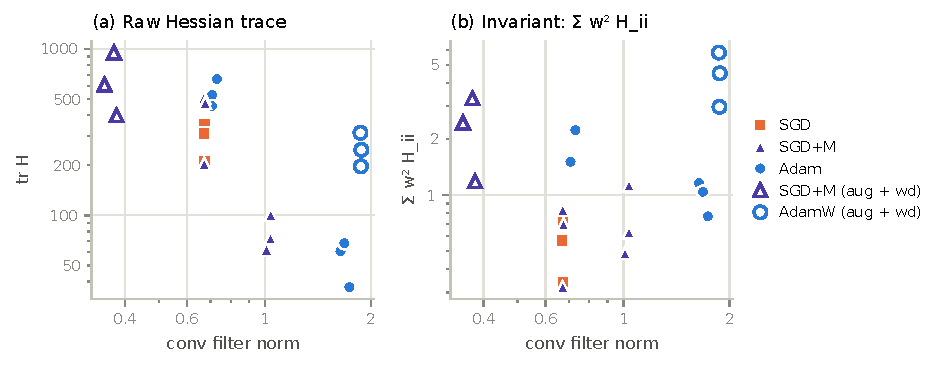
\includegraphics[width=0.85\linewidth]{fig11_resnet.pdf}
\caption{\textbf{ResNet-18 on full CIFAR-10} at training loss $0.01$ (one point per run; filled: no augmentation or weight decay, hollow: standard recipe with augmentation and weight decay; Adam with $L_2$ weight decay omitted, see text). \textbf{(a)} The raw Hessian trace falls with the conv filter norm, which the learning rate and weight decay set. \textbf{(b)} $\sum_iw_i^2H_{ii}$, invariant to every per-weight rescaling, does not; it rates Adam (filled) sharper than SGD and SGD+M at both learning rates.}
\label{fig:resnet}
\end{figure}

\textbf{ResNet-18 on full CIFAR-10.} To see whether these observations carry over to a standard architecture, we train ResNet-18, which has BatchNorm after every convolution, on the full 50k-image CIFAR-10 training set (GPU), in two sweeps with three seeds each. The first follows our protocol: no augmentation or weight decay, a constant learning rate, batch size 128, SGD ($\eta=0.1$), SGD+M ($0.01$, $0.05$) and Adam ($10^{-4}$, $5\times10^{-4}$), with checkpoints at clean training loss $1$, $0.1$ and $0.01$ (15 runs). The second is a standard recipe: random crops and flips, a cosine schedule over 60 epochs, SGD+M ($\eta=0.1$, weight decay $5\times10^{-4}$), Adam ($10^{-3}$, $L_2$ weight decay $5\times10^{-4}$) and AdamW ($10^{-3}$, decoupled weight decay $0.05$), with the same checkpoints plus the final model (9 runs). Final test accuracy is $82$--$84\%$ for SGD and SGD+M and $79$--$85\%$ for Adam in the first sweep, and $94.3$--$94.8\%$ (SGD+M), $93.4$--$93.5\%$ (AdamW) and $92.7$--$93.1\%$ (Adam) in the second. Because every convolution feeds a BatchNorm, the ReLU orbit decomposition does not apply. We use three tiers of measures instead, all computed with batch statistics on 512 clean training images: the raw trace $\tr H$; the trace at unit-norm conv filters (invariant to the BN scale symmetry), which splits $\tr H$ exactly into a BN-invariant term and a filter-norm term; and $\sum_iw_i^2H_{ii}$ and ASAM, invariant to every per-weight rescaling. The Hutchinson traces use 12 probes (median relative standard error $7$--$8\%$). The average-perturbation measures were below their sampling noise at the perturbation sizes we used (median standard error $67$--$111\%$ of the value), so we do not use them here.

Without augmentation (Fig.~\ref{fig:resnet}), the raw trace again follows the filter norms (Spearman $\rho=-0.96$, $-0.89$, $-0.62$ at losses $1$, $0.1$, $0.01$), and these are set by the learning rate: at loss $0.01$, Adam at $5\times10^{-4}$ has grown its filters to a geometric-mean norm of $1.7$, against $0.67$--$1.04$ for the other configurations. The raw verdict is accordingly all or nothing per learning-rate pairing. Adam at $5\times10^{-4}$ is rated flatter than SGD and SGD+M at $0.01$ in every seed and target, Adam at $10^{-4}$ almost never (22 of 54 seed-pairing-target triples overall). The per-weight invariant measures give one verdict: $\sum_iw_i^2H_{ii}$ rates Adam sharper in $53$ and ASAM in all $54$ triples, by a factor of $2.1$--$2.9$ against SGD for $\sum_iw_i^2H_{ii}$ (geometric means). At loss $0.01$ the exact split of the Adam/SGD trace ratio is $-0.75$ bits $=+0.14$ (BN-invariant term) $-0.89$ (filter norms): the norms hide the difference that the invariant measures see. The pattern of the BatchNorm MLP therefore replicates (raw measures read off learning-rate-dependent norms and their verdict depends on the pairing, while invariant measures give one verdict), but the direction of the invariant verdict does not: in ResNet-18, Adam is the sharper one.

With the standard recipe, the raw trace rates AdamW flatter than SGD+M in all three seeds at loss $0.1$, at loss $0.01$ and at the end of training, by $0.35$--$2.30$ bits ($1.3$--$4.9\times$). The split attributes most of this to AdamW's larger filters (filter-norm term $-1.0$ to $-1.5$ bits; geometric-mean filter norm $1.83$--$1.88$ against $0.34$--$0.44$). The per-weight invariant measures do not support the raw verdict: $\sum_iw_i^2H_{ii}$ and ASAM each rate AdamW sharper in 7 of these 9 seed-target pairs, some by small margins. With three seeds we report only that the raw advantage is a filter-norm effect, not a reversal. Adam with coupled $L_2$ weight decay behaves differently again: it drives the filters of the deeper layers to zero, so that in 5 to 8 of the 20 convolutions more than half of the filters have norm below $0.01$. This never happens for AdamW or SGD+M and matches the filter-level sparsity reported for Adam with $L_2$ regularization and BatchNorm \citep{mehta2019filter}. A zero filter feeding a BatchNorm layer makes the curvature depend on BatchNorm's $\epsilon$, so we leave this configuration out of the comparison.

%===============================================================================


\section{Measure definitions}\label{app:measures}
All measures use mean cross-entropy on a fixed evaluation subset of 4096 training examples (CNN: 1024; $\mathrm{diag}(G)$ for the CNN uses its first 512), shared by all models. Random perturbations use common random numbers across models.
\begin{itemize}[leftmargin=1.2em,itemsep=1pt]
\item \emph{Original metric}: $\big(\mathbb{E}_\varepsilon L_{\mathrm{test}}(w+\sigma\varepsilon)-L_{\mathrm{test}}(w)\big)/L_{\mathrm{test}}(w)$, $\varepsilon\sim\mathcal N(0,I)$ on all parameters, $\sigma=0.01$, 10 draws, full test set.
\item \emph{Isotropic average}: $\mathbb{E}L(w+\sigma\varepsilon)-L(w)$, $\sigma\in\{0.003,0.01,0.03\}$, 16 draws; we report $\sigma=0.01$.
\item \emph{Filter-normalized average} \citep{li2018visualizing}: each output unit's (or filter's) row of a Gaussian direction is rescaled to the norm of the corresponding weight row; biases are not perturbed; scale $\in\{0.01,0.03,0.1\}$, 16 draws; we report $0.03$. Invariant to scaling a row, not to neuron rescaling (\S\ref{sec:protocol}).
\item \emph{Multiplicative average}: $\delta=\sigma|w|\odot\varepsilon$, $\sigma\in\{0.01,0.03,0.1\}$; we report $0.03$.
\item \emph{Hessian trace}: Hutchinson with 20 Rademacher probes. $\tr G$: exact, from the exact diagonal Gauss--Newton matrix; for the MLPs and the CNN it equals the Hessian trace (Lemma~\ref{lem:diag}), of which the Hutchinson value is a stochastic estimate.
\item $\lambda_{\max}$: Lanczos (\texttt{scipy eigsh}, tolerance $10^{-3}$) on Hessian--vector products.
\item \emph{SAM worst-case}: $\max_{\|\delta\|_2\le0.05}L(w+\delta)-L(w)$ by 10 steps of normalized projected gradient ascent with step $0.4\rho$. \emph{ASAM worst-case} \citep{kwon2021asam}: the same with $\|\delta/|w|\|_2\le0.5$.
\item $\MS_p$: coordinate descent until the relative change is below $10^{-10}$. The minimum-norm point: alternating per-unit balancing until $\max_j|\log c_j|<10^{-7}$.
\end{itemize}
Verification: the fast MLP $\mathrm{diag}(G)$ matches a per-sample implementation to $2{\times}10^{-8}$, which matches a brute-force $J^\top SJ$ to $3{\times}10^{-8}$. Rescalings preserve the network output to $3{\times}10^{-6}$. The analytic transport of $\mathrm{diag}(G)$ matches recomputation to $2{\times}10^{-7}$ (MLP) and $3{\times}10^{-7}$ (CNN). $\MS_p$ was never beaten by the raw, minimum-norm or random rescalings tested. Under random rescalings (log-scale s.d.\ $1$), the multiplicative average, ASAM and $\sum_iw_i^2H_{ii}$ change by less than $2{\times}10^{-4}$ relative (the residual comes from BatchNorm's $\epsilon$, which moves the loss itself by as much), both for ReLU neuron rescaling in the MLP and for the two symmetries of the BatchNorm MLP (\S\ref{sec:bn}); filter-normalized sharpness changes by factors of $9.5$ and $19$ under the neuron and BN-affine rescalings.

\section{Drift experiment: all optimizers}\label{app:drift}
\begin{table}[h]
\centering
\small
\caption{Drift experiment (CIFAR-10 MLP, $32{\times}32$ inputs, batch size 128, 20 epochs, mean of two seeds). $D^{(1)}$ and $D^{(2)}$ are the cumulative first- and second-order drift terms of~\eqref{eq:decomp}, averaged over first-layer units; $E$ is the final orbit excess. The decomposition closes to $\le1.3\times10^{-6}$ in every run.}
\label{tab:drift}
\begin{tabular}{llccccc}
\toprule
Optimizer & $\eta$ & final train loss & $D^{(1)}$ & $D^{(2)}$ & imbalance (L1) & $E$\\
\midrule
SGD & $0.01$ & 1.44 & $0.0000$ & 0.0023 & 0.31 & 1.70\\
SGD & $0.03$ & 0.92 & $0.0000$ & 0.064 & 0.32 & 2.31\\
SGD & $0.1$ & 0.57 & $0.0000$ & 0.577 & 0.47 & 1.78\\
SGD+M & $0.001$ & 1.45 & 0.0023 & 0.0001 & 0.31 & 1.68\\
SGD+M & $0.003$ & 0.90 & 0.048 & 0.0027 & 0.30 & 2.41\\
SGD+M & $0.01$ & 0.46 & 0.576 & 0.032 & 0.48 & 1.99\\
SAM (SGD+M, $r=0.05$) & $0.003$ & 1.10 & 0.069 & 0.0015 & 0.36 & 1.80\\
\midrule
Adam & $3{\times}10^{-5}$ & 1.50 & 0.067 & 0.0003 & 0.41 & 1.14\\
Adam & $10^{-4}$ & 1.13 & 0.255 & 0.0032 & 0.55 & 1.14\\
Adam & $3{\times}10^{-4}$ & 0.62 & 1.076 & 0.027 & 0.86 & 1.12\\
Adam & $10^{-3}$ & 0.27 & 6.151 & 0.261 & 1.40 & 1.19\\
RMSprop & $3{\times}10^{-5}$ & 1.37 & 0.114 & 0.025 & 0.48 & 1.11\\
RMSprop & $10^{-4}$ & 0.96 & 0.397 & 0.272 & 0.78 & 1.10\\
RMSprop & $3{\times}10^{-4}$ & 0.52 & 1.149 & 2.186 & 1.27 & 1.28\\
signSGD & $3{\times}10^{-5}$ & 1.57 & 0.052 & 0.0042 & 0.40 & 1.15\\
signSGD & $10^{-4}$ & 1.25 & 0.149 & 0.047 & 0.51 & 1.14\\
signSGD & $3{\times}10^{-4}$ & 0.81 & 0.359 & 0.423 & 0.78 & 1.14\\
\bottomrule
\end{tabular}
\end{table}
For sign descent and RMSprop at larger learning rates the second-order term becomes comparable to the first-order one. Each coordinate moves by $\approx\eta$, so $\|u_{a_j}\|^2-\|u_{c_j}\|^2\approx\eta^2(d_{\mathrm{in}}-d_{\mathrm{out}})$, which is a second, fan-in-driven contribution in the same direction.

\section{Robustness to the learning-rate pairing}\label{app:lrpairs}
\begin{table}[h]
\centering
\small
\caption{$P(\text{Adam rated flatter than SGD})$ for each pair of base learning rates, pooled over the $3\times3$ batch-size pairs, three seeds and training losses $\{0.1,0.03,0.01\}$ (81 pairs per cell).}
\label{tab:lrpairs}
\begin{tabular}{cc cccc cccc}
\toprule
& & \multicolumn{4}{c}{CIFAR-10} & \multicolumn{4}{c}{MNIST}\\
\cmidrule(lr){3-6}\cmidrule(lr){7-10}
Adam $\eta_0$ & SGD $\eta_0$ & $\tr G$ & orig. & $\MS_1$ & filter & $\tr G$ & orig. & $\MS_1$ & filter\\
\midrule
$10^{-4}$ & $0.01$ & 1.00 & 1.00 & 0.00 & 0.02 & 0.84 & 0.91 & 0.42 & 0.26\\
$10^{-4}$ & $0.03$ & 0.06 & 0.00 & 0.00 & 0.05 & 0.19 & 0.58 & 0.00 & 0.10\\
$3{\times}10^{-4}$ & $0.01$ & 1.00 & 1.00 & 0.27 & 0.05 & 0.98 & 0.93 & 0.88 & 0.54\\
$3{\times}10^{-4}$ & $0.03$ & 0.60 & 0.59 & 0.07 & 0.09 & 0.68 & 0.83 & 0.21 & 0.33\\
\bottomrule
\end{tabular}
\end{table}

\section{Calibration of learning rates}\label{app:calibration}
Before the main sweeps we trained every optimizer with four learning rates and three batch sizes for up to 200 epochs (seed 0, no measures). Table~\ref{tab:calib} reports the epoch at which the training loss first fell below $0.01$, or the final loss in parentheses if it did not. No single learning rate trains stably at every batch size: SGD at $\eta=0.1$, for example, fails at $B=32$ but works at $B=512$. We therefore use square-root scaling, $\eta=\eta_0\sqrt{B/32}$, with the base rates $\eta_0\in\{0.01,0.03\}$ (SGD), $\{10^{-3},3{\times}10^{-3}\}$ (SGD+M, SAM) and $\{10^{-4},3{\times}10^{-4}\}$ (Adam). Every main-sweep run reached all loss targets within 300 epochs.
\begin{table}[h]
\centering
\small
\caption{Calibration: epochs to reach training loss $0.01$ (final loss in parentheses if not reached in 200 epochs).}
\label{tab:calib}
\begin{tabular}{llccc@{\qquad}llccc}
\toprule
\multicolumn{5}{c}{CIFAR-10 MLP} & \multicolumn{5}{c}{MNIST MLP}\\
\cmidrule(lr){1-5}\cmidrule(lr){6-10}
Opt. & $\eta$ & $B{=}32$ & $128$ & $512$ & Opt. & $\eta$ & $B{=}32$ & $128$ & $512$\\
\midrule
SGD & 0.01 & 67 & (0.01) & (0.85) & SGD & 0.01 & 61 & (0.02) & (0.16)\\
SGD & 0.03 & 49 & 94 & (0.10) & SGD & 0.03 & 20 & 80 & (0.03)\\
SGD & 0.1 & (0.77) & 56 & 163 & SGD & 0.1 & 9 & 24 & 98\\
SGD & 0.3 & (2.30) & (0.79) & (1.23) & SGD & 0.3 & 19 & 10 & 35\\
SGD+M & 0.001 & 67 & (0.01) & (0.86) & SGD+M & 0.001 & 61 & (0.02) & (0.16)\\
SGD+M & 0.003 & 63 & 80 & (0.04) & SGD+M & 0.003 & 21 & 81 & (0.04)\\
SGD+M & 0.01 & (0.64) & 63 & 98 & SGD+M & 0.01 & 9 & 26 & 103\\
SGD+M & 0.03 & (2.29) & (0.50) & 75 & SGD+M & 0.03 & 20 & 11 & 36\\
SAM & 0.001 & 129 & (0.05) & (1.02) & SAM & 0.001 & 61 & (0.01) & (0.16)\\
SAM & 0.003 & 105 & 129 & (0.12) & SAM & 0.003 & 23 & 77 & (0.03)\\
SAM & 0.01 & (0.32) & 93 & 161 & SAM & 0.01 & 12 & 27 & 96\\
SAM & 0.03 & (1.60) & (0.23) & 106 & SAM & 0.03 & 13 & 12 & 35\\
Adam & 3e-5 & (0.02) & (0.41) & (0.91) & Adam & 3e-5 & 161 & (0.06) & (0.17)\\
Adam & 1e-4 & 97 & 164 & (0.13) & Adam & 1e-4 & 50 & 112 & (0.03)\\
Adam & 3e-4 & 60 & 81 & 158 & Adam & 3e-4 & 20 & 44 & 99\\
Adam & 1e-3 & (0.08) & 52 & 70 & Adam & 1e-3 & 16 & 18 & 38\\
\bottomrule
\end{tabular}
\end{table}

\section{Edge-of-stability observation}\label{app:eos}
In pilot runs with the original raw inputs (CIFAR-10 MLP, batch size 128), SGD's $\lambda_{\max}$ tracked the stability threshold $2/\eta$: $17$--$22$ at $\eta=0.1$ (threshold $20$), $47$--$74$ at $\eta=0.03$ ($67$), and $187$--$252$ at $\eta=0.01$ ($200$). Sharpness comparisons at a single learning rate per optimizer therefore largely compare learning rates.



\end{document}
